\documentclass[conference]{IEEEtran}
\usepackage{cite}
\usepackage{amsmath,amssymb,amsfonts}
\usepackage{algorithmic}
\usepackage{graphicx}   %插入图片的宏包
\usepackage{float}      %设置图片浮动位置的宏包
\usepackage{subfigure}  %插入多图时用子图显示的宏包
\usepackage{textcomp}
\usepackage{xcolor}
\usepackage[hyphens]{url}
\usepackage{multirow}
\usepackage{array}
\usepackage{makecell}
\usepackage{booktabs}
\usepackage{enumerate}
% \usepackage{algorithm}
% \usepackage{algorithmic}
\usepackage[ruled]{algorithm2e}

\def\BibTeX{{\rm B\kern-.05em{\sc i\kern-.025em b}\kern-.08em
    T\kern-.1667em\lower.7ex\hbox{E}\kern-.125emX}}

% Ensure letter paper
\pdfpagewidth=8.5in
\pdfpageheight=11in

%%%%%%%%%%%---SETME-----%%%%%%%%%%%%%
\newcommand{\iscasubmissionnumber}{NaN}
%%%%%%%%%%%%%%%%%%%%%%%%%%%%%%%%%%%%

\pagenumbering{arabic}

%%%%%%%%%%%---SETME-----%%%%%%%%%%%%%
\title{On Optimizing Large Integer Modular Multipliers on FPGA}
% \author[]{Tianrui Li}
%%%%%%%%%%%%%%%%%%%%%%%%%%%%%%%%%%%%

\begin{document}
\maketitle
\thispagestyle{plain}
\pagestyle{plain}

%%%%%% -- PAPER CONTENT STARTS-- %%%%%%%%

\begin{abstract}
\textcolor{black}{
In recent years, with the steady inroads of FPGAs into data centers, many applications in cryptography have been offloaded onto FPGAs. Among these applications, modular multiplication has a pivotal role. Except for the simplest block ciphers, modular multiplication is the most computationally intensive part of almost all modern applications in cryptography, including public-key cryptography, post-quantum cryptography, fully homomorphic encryption, and zero-knowledge proofs. However, pipelined implementation of long modular multipliers on FPGAs requires hundreds of DSP and thousands of LUT resources. Therefore, optimization of the modular multiplier can significantly reduce the area and power overhead of the application. In this work, we build a taxonomy of a modular multiplier's specific configurations and accurately estimate each configuration's overhead through a primitive-based design methodology. Based on this model, we propose and implement novel algorithms that automatically search for an overall solution based on the user's FPGA budget and generate RTL-level descriptions. By eliminating functional redundancy, our algorithm generates customized modular multipliers with over 60\% area reduction compared to general-purpose modular multipliers. Furthermore, by exploiting compressor trees and primitive level optimization, our generated results achieve over 20\% area reduction on constant multipliers while maintaining the same frequency as in other works.
}
\end{abstract}

\section{Introduction}
 
\graphicspath{ {./images/} }
% 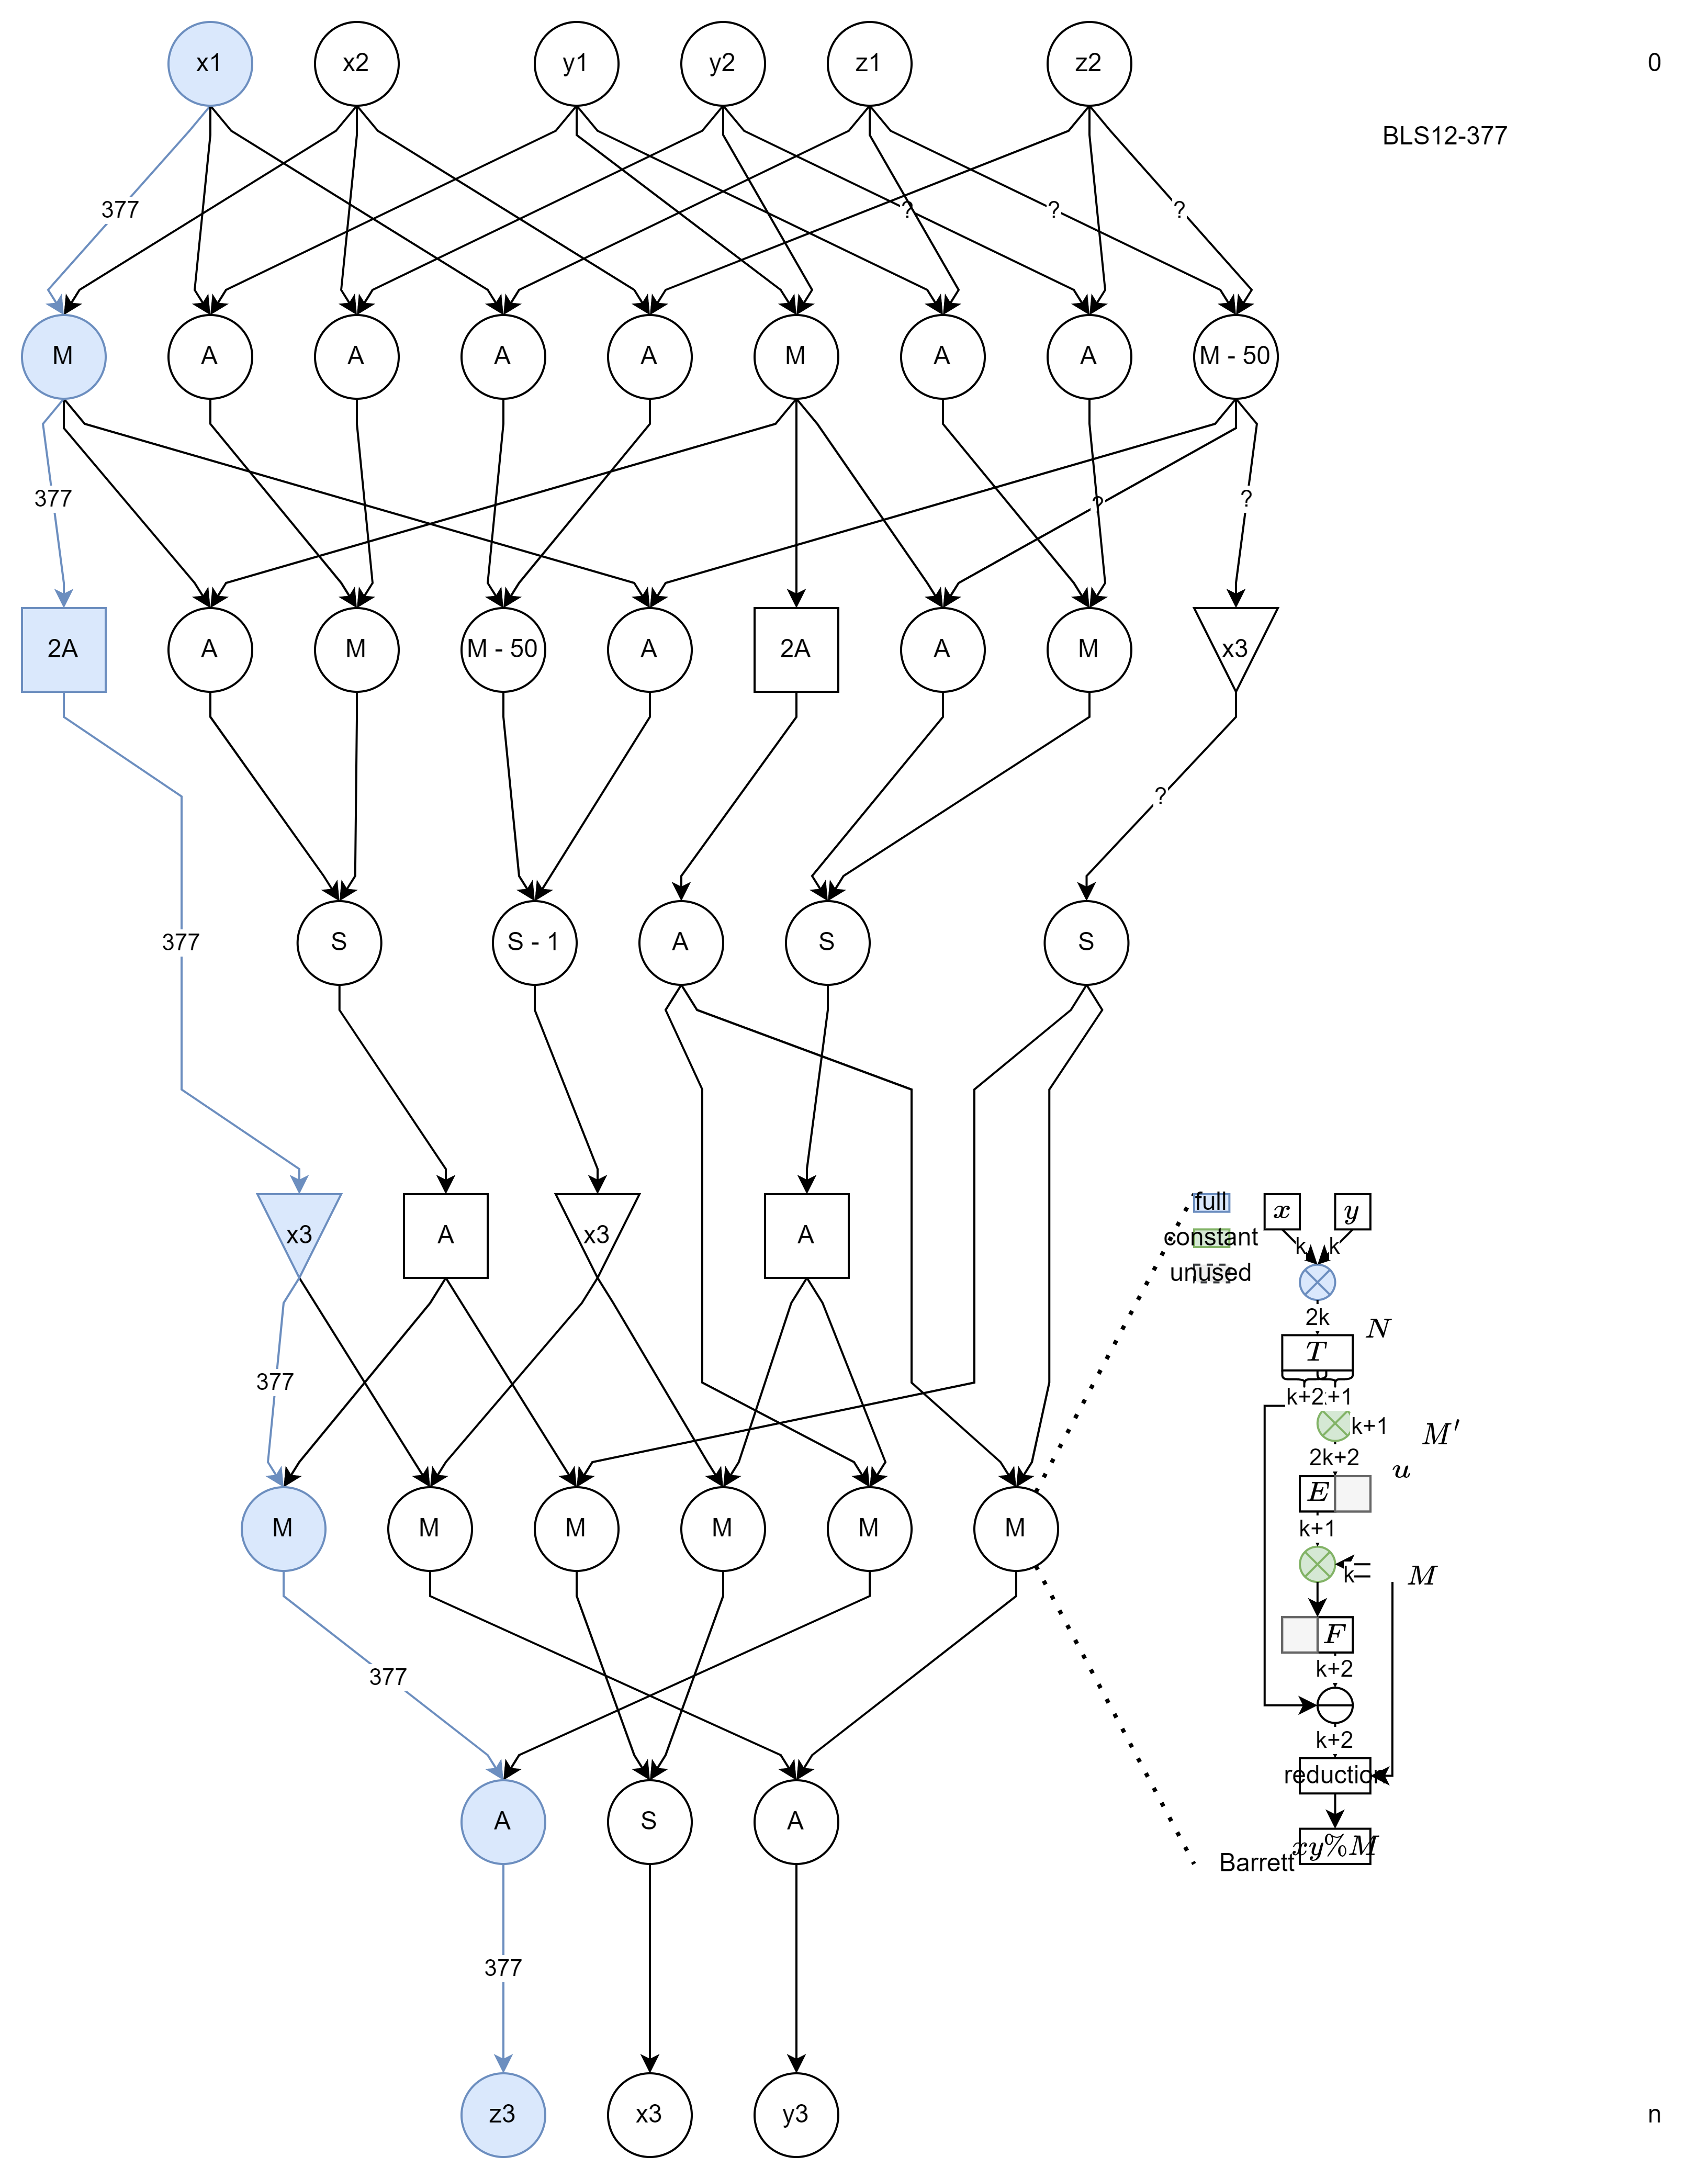
\includegraphics{Untitled.png}
% FIXME: Make a better graph

% % 单栏图片
% \begin{figure}[htbp]   %单栏图片用{figure}; 双栏用{figure*},加个星号
% 	\centering
% 	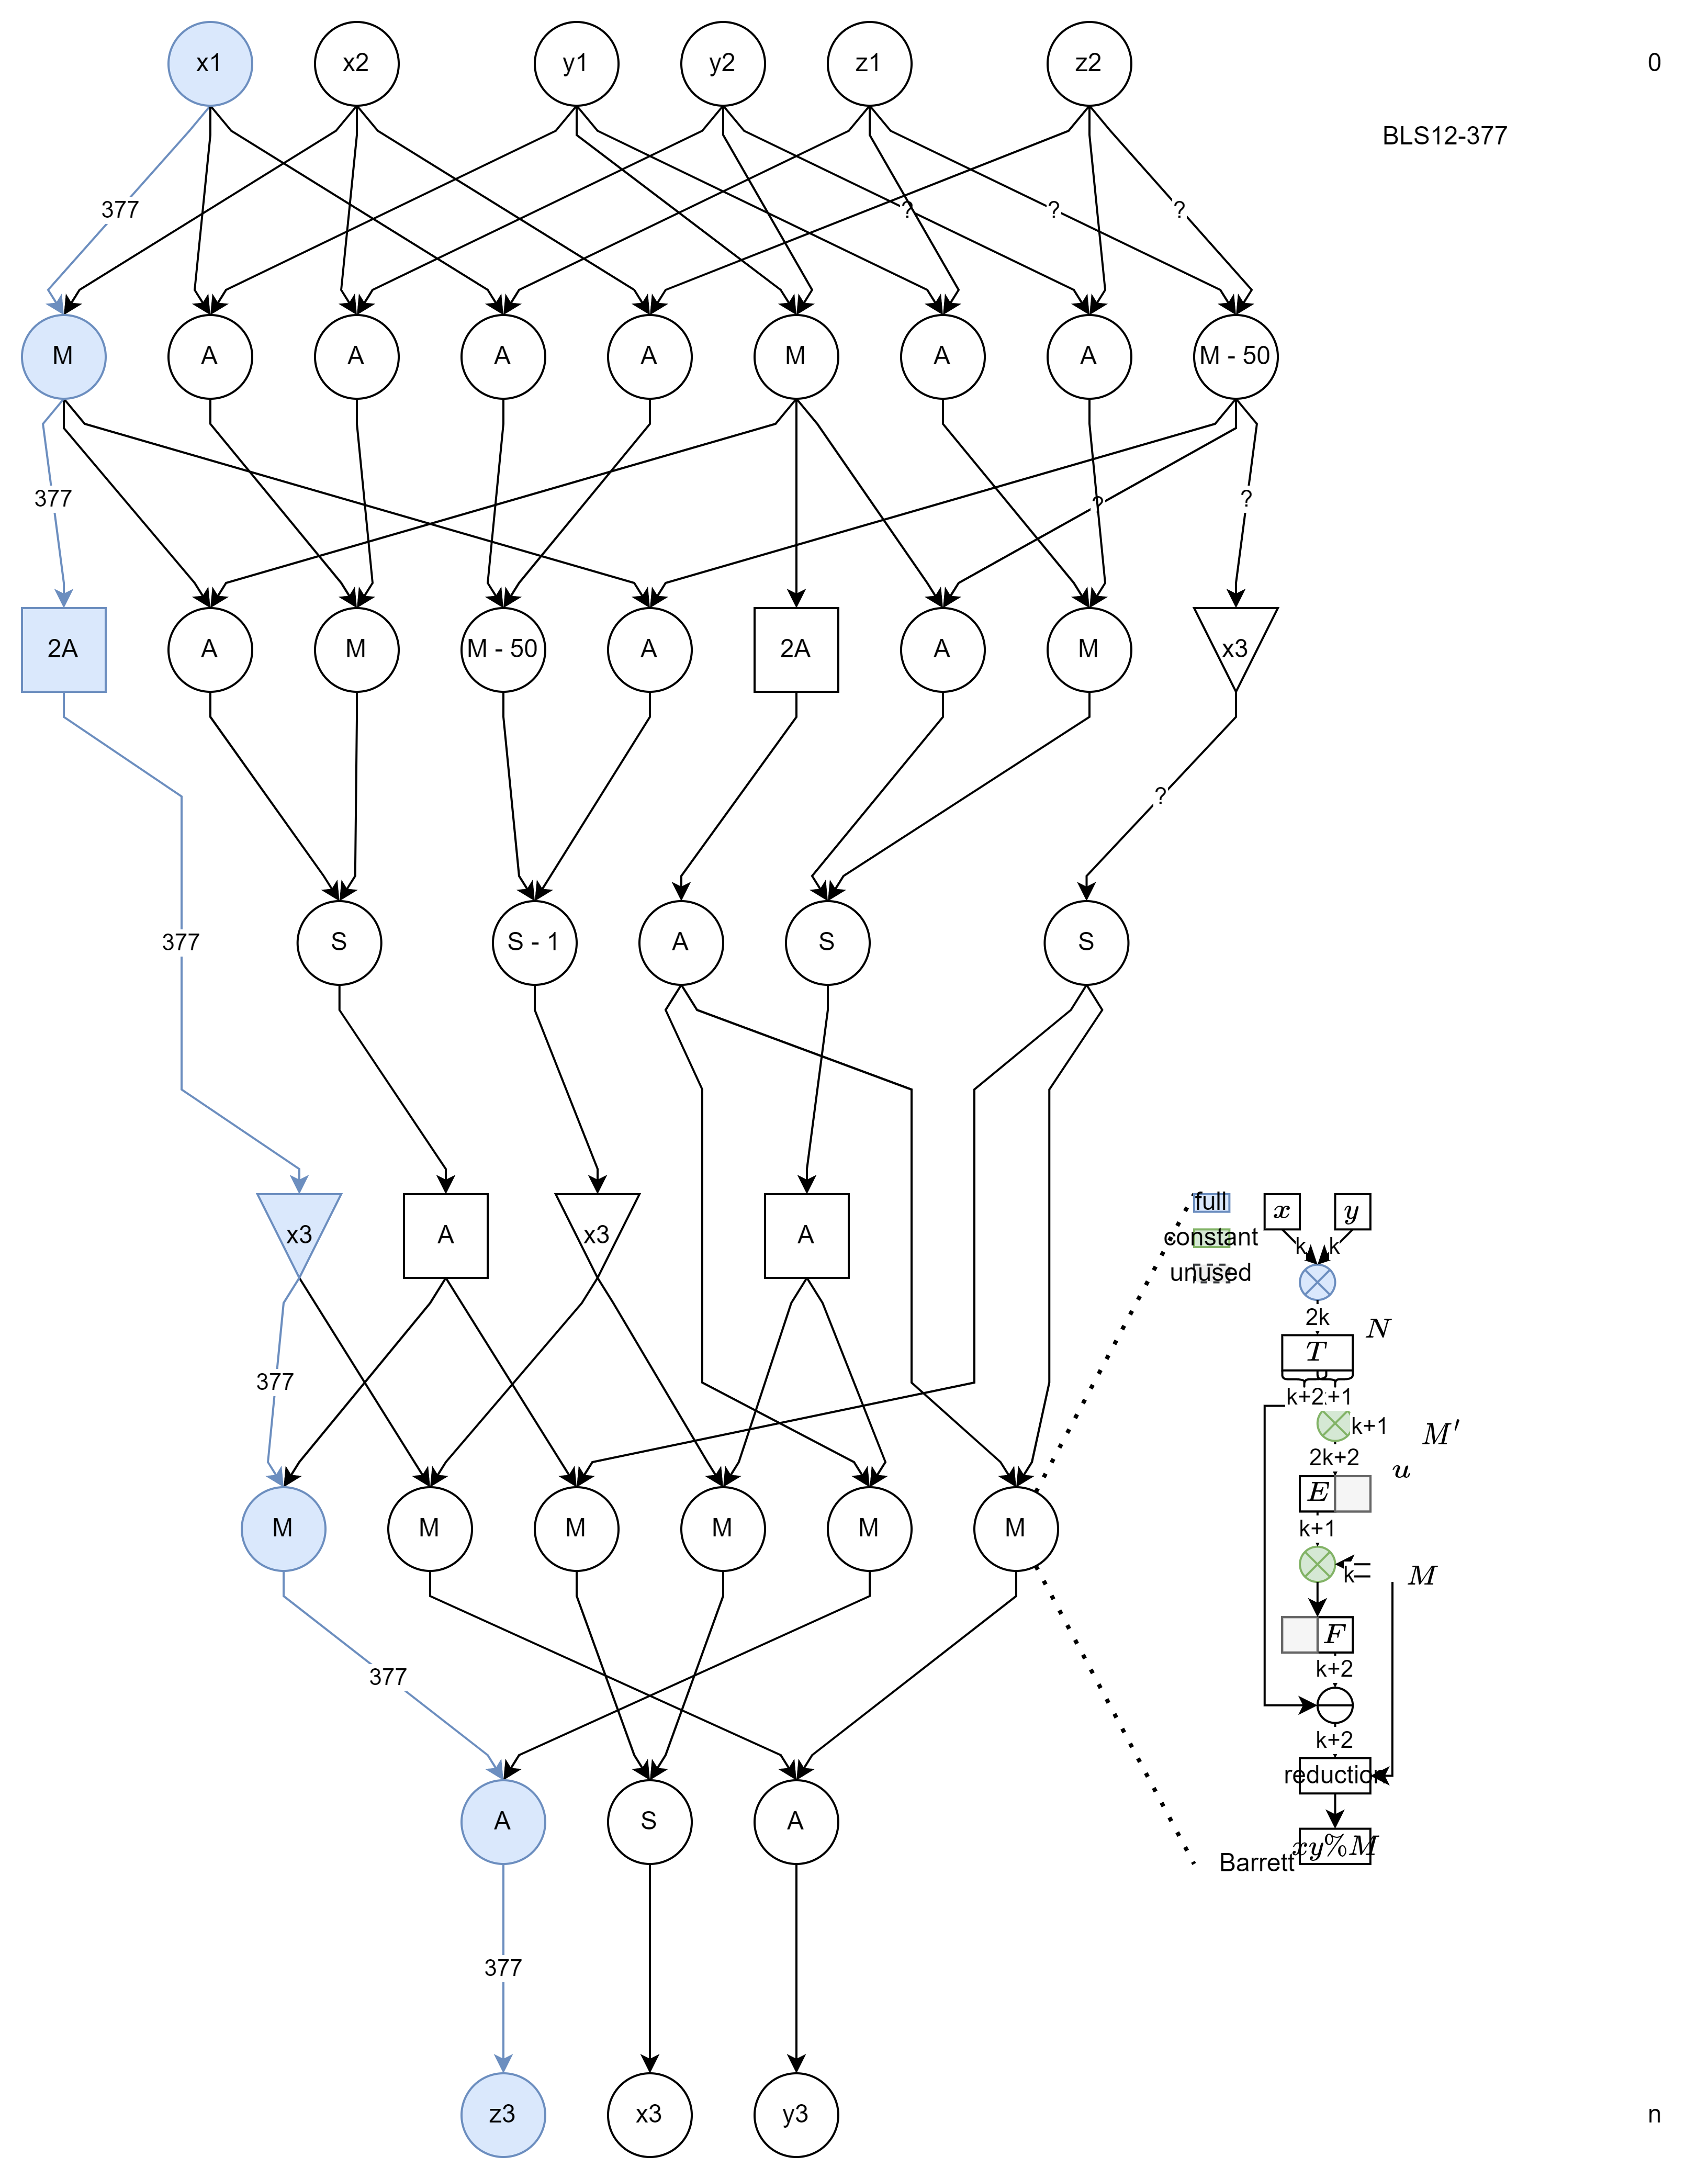
\includegraphics[width=\linewidth,scale=1.00]{Untitled.png}    %[]里面的参数自己可根据需要调整
% 	\caption{Please write what you want.}
% 	\label{FigureOne}
% \end{figure}

With the wide adoption of FPGAs in data centers, one of major applications of FPGAs is to accelerate cryptography applications, where finite-field arithmetic is one kind of heavy workload on FPGAs due to its wide application in codecs and cryptography.


In addition to classical symmetric (e.g., AES) and asymmetric (e.g., RSA) ciphers, recent applications, including post-quantum cryptography, fully homomorphic encryption, and zero-knowledge proofs take long finite-field operations as their computational primitives as well. Among these operations, the most important one is modular multiplication, which accounts for more than 90\% of the computational overhead in each of these applications.

Montgomery's modular multiplication ~\cite{Montgomery}  and Barrett's reduction ~\cite{Implementing_the_Rivest_Shamir_and_Adleman_public_key} are the two most prominent methods for implementing modular multiplication. Although the principles are different, they share highly similar datapaths, with the main components being a long full multiplication and two constant multiplications. Therefore, for their implementation, similar optimization techniques can be used. In previous works, due to the limitations of FPGA resources and application scenarios, most of the works focused on reducing silicon area or total power consumption through folding (hardware reuse). However, as FPGAs are widely used in data centers, work geared towards high throughput and energy efficiency is beginning to emerge.

In this paper, we aim to provide a comprehensive and detailed discussion of the design techniques of long modular multipliers on FPGAs and finally implement an efficient generator for modular multipliers. In this paper, two multiplication types: full multiplication and constant multiplication; two divide-and-conquer techniques: Karatsuba ~\cite{Multiplication_of_multidigit_numbers_on_automata} and Schoolbook; and two addition implementation techniques: carry-propagation (CPA) addition and compressor tree (carry-save addition, CSA), are incorporated into the same "bit heap" based framework. In this framework, these techniques distribute the unevaluated bits to three categories: addition, multiplication, and the compressor tree, each having a different cost function. This way, the cost and benefits of these techniques can be quantified, which will drive a brand-and-bound algorithm to find the best mapping from the algorithm to these computational primitives by searching over the decision tree. Furthermore, we implement a toolchain to automatically generate the pipeline for this mapping to achieve the smallest possible latency and register consumption under a specific frequency constraint. Finally, we combined all these tools into a SpinalHDL-based modular multiplier generator, which is open source on GitHub


\textcolor{black}{
In general, the contributions of this paper are as follows:
\begin{enumerate}[1.]
    \item We propose a taxonomy of implementations for long (modular) multipliers, under which generators can accurately implement non-redundant custom (modular) multipliers, thus reducing the area overhead.
    \item We propose a taxonomy that classifies the primitives used to implement multiplication on FPGAs into three categories and build an accurate cost-and-benefit model for these primitives as the basis for subsequent search algorithms.
    \item We incorporated various previously proposed, unrelated design techniques, including rectangular Karatsuba and truncated Barrett algorithm, into the same generator framework and give a quantitative performance analysis of these techniques under our model.
    \item We propose a branch-and-bound algorithm and an ILP-based method to generate an overall solution for implementing long (modular) multipliers on a specific device. As a result, the user only needs to provide an FPGA resource budget and a specific configuration of target (modular) multipliers. This result can be obtained within minutes, even for the largest FPGAs available.
    \item We utilize Scala and SpinalHDL to complete an open-source, out-of-the-box modular multiplier generator.
\end{enumerate}
}

% \section{BACKGROUND AND MOTIVATION}

\section{RELATED WORK}

\subsection{Existing Works aiming at Small Area}

\textcolor{black}{
For a long time, a long modular multiplier is often folded, which is limited by the capacity of the previous FPGA on the one hand and the actual demand on the other. ~\cite{Comparison_of_Montgomery_and_Barrett_modular_multipliers_on_FPGAs} compares Mont and Barrett, ~\cite{Automatic_Generation_of_Modular_Multipliers_for_FPGA_Applications} studies the automatic generation of folded modular multipliers up to 256 bits. ~\cite{High_Throughput_FPGA_Implementation_of_256_bit_Montgomery_Modular_Multiplier} implements a folded modular multiplier base on Karatsuba multiplier, which implements the three multiplications in Barrett through a pipelined Karatsuba multiplier. ~\cite{A_High_Performance_Full_Word_Barrett_Multiplier_Designed_for_FPGAs_with_DSP_Resources} use six 48-bit multipliers to calculate a 528-bit modular multiplication.
}


\subsection{Existing Works aiming at High Throughput}
\textcolor{black}{
However, in recent years, with the increase of FPGA capacity and the emergence of some applications that require a large amount of computing (such as zero-knowledge proof, fully homomorphic encryption, Etc.), some high-throughput-oriented work has gradually emerged. Several or even dozens of pipelined long modular multipliers are implemented in these works. For example, towards Classical Elliptic Curve Cryptography, in article ~\cite{A_High_performance_ECC_Processor_over_Curve448_based_on_a_Novel_Variant_of_the_Karatsuba_Formula_for_Asymmetric_Digit_Multiplier,  High_Speed_and_Unified_ECC_Processor_for_Generic_Weierstrass_Curves_over_GFp_on_FPGA,Fast_Small_and_Area_Time_Efficient_Architectures_for_Key_Exchange_on_Curve25519}, invariably design a pipelined modular multiplier for specific elliptic curve. In the zero-knowledge proof oriented works, parallelism is exploited more thoroughly. In PipeMSM ~\cite{PipeMSM}, they implement 2 fully flattened elliptic curve addition units on a single FPGA, including 24 377-bit modular multipliers. In CycloneMSM ~\cite{FPGA_Acceleration_of_Multi_Scalar_Multiplication_CycloneMSM}, they also implement a flattened elliptic curve addition unit containing 8 377-bit modular multipliers.
}

\subsection{Karatsuba, Bit heap and Compressor Tree}

\textcolor{black}{
Another important basis for  this paper is the adoption of Karatsuba algorithm and compressor tree. Karatsuba ~\cite{Multiplication_of_multidigit_numbers_on_automata}
 and compressor tree ~\cite{Advanced_Compressor_Tree_Synthesis_for_FPGAs} (i.e. carry-save addition) are two mature methods that have been widely used in the implementation of arithmetic hardware. In the past decade, there have been some new progress worth mentioning for their implementation on FPGAs.
}

\textcolor{black}{
For a long time, CSA was mainly used on ASIC and was considered unsuitable for FPGA implementation. However, at present, the preparation for its application on FPGA has been sufficient, and one of the milestone works is ~\cite{Arithmetic_core_generation_using_bit_heaps}. In this work, Brunie et al. propose the bit heap model, under which multiplication and (multi-input) addition can be regarded as the same operation  - compression. The computational unit which implements multiplication and addition is abstracted as a compressor and defined by the bit heap of its inputs and outputs. This model enables the "computational power" of all computational units on the FPGA to be quantitatively measured on a unified scale. At the same time, the bit heap also provides an excellent object-oriented model. Bit heap was initially implemented in flopoco [FIXME], their open-source library of FPGA operators, and we implement this model independently in our open-source library, Chainsaw.
}

\textcolor{black}{
In terms of Karatsuba, ~\cite{Karatsuba_with_Rectangular_Multipliers_for_FPGAs} proposed a method for efficiently utilizing the rectangular multiplier on the FPGA. While~\cite{IMpress_Large_Integer_Multiplication_Expression_Rewriting_for_FPGA_HLS} proposed a method for Karatsuba architecture search based on expression rewriting.
}


\section{PRELIMINARIES}

\subsection{Karatsuba Algorithm}

\subsubsection{Fundamentals of Karatsuba}

In the hardware implementation, to accomplish the multiplication of large numbers, we need to continuously perform decompositions on operands until some multiplier can directly process their widths and then combine the results of these multiplications in a weighted form. A natural way to do this in binary form is to divide the original width into n parts. When $n=2$, the formula is as follows:
\begin{equation}
    \begin{split}
        \begin{aligned}A \times B &=\left(a_1 2^W+a_0\right)\left(b_1 2^W+b_0\right) \\
        &={a_1 b_1} 2^{2 W}+({a_1 b_0}+{a_0 b_1}) 2^W+{a_0 b_0}\end{aligned}
    \end{split} 
\end{equation}


We refer to this method as the \textbf{schoolbook} method. \textbf{Karatsuba}'s algorithm is the first multiplication algorithm with sub-quadratic complexity. It trades multiplications for additions when compared to the schoolbook method. When $n=2$, Karatsuba's method reduces four multiplications to three by reusing the products $a_0b_0$ and $a_1b_1$. The premise of this reuse is that the weights of the cross-term $a_1b_0$ and $a_0b_1$ are the same. In Figure \ref{Figure1}, this is shown by the fact that the cross terms $M_1$ and $M_2$ are aligned vertically.
\begin{equation}
    \begin{split}
        a_1 b_0+a_0 b_1=\left(a_0+a_1\right)\left(b_0+b_1\right)-{a_0 b_0}_{}-{a_1 b_1}_{}
    \end{split} 
\label{basic-kara}
\end{equation}

\textcolor{black}{
We refer to the calculation contained on the right hand side of the formula \ref{basic-kara} as a \textbf{basic Karatsuba calculation} with inputs $a_1, a_0, b_1, b_0$ and outputs $a_1b_1, a_0b_0$ and $a_1b_0 + b_1a_0$. In the later section, we optimize this operation based on DSP primitives.
}

\textcolor{black}{
$2$-split Karatsuba can be generalized to $n$-split Karatsuba. Taking $3$-split as an example, in Figure \ref{Figure1}, the diagonal product terms $M_0$, $M_4$ and $M_8$ are reused, and the calculation can be done in two steps: The first is the calculation of  product terms on the diagonal, and the second is the calculation of cross-terms which are colored in Figure \ref{Figure1}.b, cross-terms of same color can be computed by only one extra multiplication taking advantage of the diagonal terms. 
}

For n-split case, the number of sub-multiplications is the size of the upper triangle, including the diagonal, i.e., $n(n+1) \over 2$, while schoolbook method takes $n^2$. n-split Karatsuba can be utilized recursively to obtain higher compression ratios. An example is that two 2-split Karatsuba decompositions can also implement the multiplier implemented by a 4-split Karatsuba decomposition. The cost of the recursive n-split Karatsuba algorithm is shown in formula \ref{n-split Karatsuba}.
\begin{equation}
    \begin{split}
        T(W)&={n(n+1)\over 2} T(W/n)+O(W)
    \end{split} 
\label{n-split Karatsuba}
\end{equation}

According to the main theorem, the asymptotic complexity of multiplication and addition are both $T(W)=\Theta\left(W^{\log {(n+1)\over 2}}\right)$. The smaller the $n$, the better the asymptotic complexity. But smaller n increase the number of nested layers of the whole structure, leading to a large latency. In addition, by introducing $n$-split instead of just $2$-split, a decomposition scheme can end up at a width closer to the target, avoiding excessive padding.

\begin{figure}[htbp]   %单栏图片用{figure}; 双栏用{figure*},加个星号
	\centering
	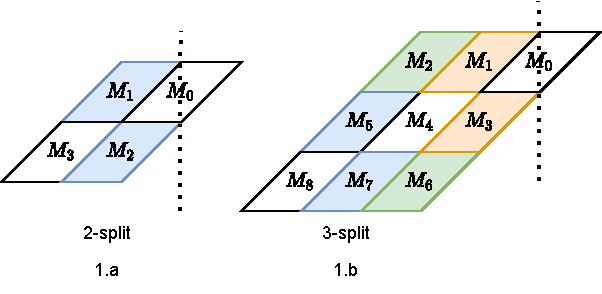
\includegraphics[width=\linewidth,scale=1.00]{fig1.pdf}    %[]里面的参数自己可根据需要调整
	\caption{2-split Karatsuba and n-split Karatsuba}
	\label{Figure1}
\end{figure}

\subsubsection{Rectangular Karatsuba}

~\cite{Karatsuba_with_Rectangular_Multipliers_for_FPGAs} introduces the rectangular Karatsuba method to better exploit the non-square-shaped embedded multipliers on modern FPGAs and to better match the case where the target size of the solution is rectangular. A short review is given below.

In ~\cite{Karatsuba_with_Rectangular_Multipliers_for_FPGAs}, assuming that in a Karatsuba decomposition, the size of the sub-multipliers are $\left(W_A, W_B\right)$, and its greatest common divisor is $W=\operatorname{gcd}\left(W_A, W_B\right)$, and note that $M=W_A / W$, $N=W_B / W$. Then on a tiling scale of at least $(N+1)\times (M+1)$ sub-multipliers, there exists combinations that can use Karatsuba's method. In Figure \ref{Figure2}, embedded multipliers of size  $(16,24)$ (2:3) are used.  A pair of cross terms $M_1, M_2$(black) can be utilized by Karatsuba's method on a mesh with a size of at least $3\times 4$. The $M0, M1, M2$, and $M3$ form a basic Karatsuba's calculation, which is defined in Formula \ref{basic-kara}

~\cite{Karatsuba_with_Rectangular_Multipliers_for_FPGAs} gives various examples of using rectangular Karatsuba on different-size meshes, but when the design goal is a square multiplier, the most efficient way is a combination of $n$-split and rectangular. In Figure \ref{Figure2}, we use a multiplier with a size ratio 2:3, where a block of $3/times 2$ multipliers forms a square. We tile $n \times n$ such blocks, and the sub-multipliers at the same position in each block form a set of $n$-split Karatsuba decomposition. A 3-tuple $$\left(W_A, W_B, n\right)$$ can fully define such a Karatsuba decomposition:

The size of this 3-tuple is $nNMW \times nNMW$, and the number of sub-multipliers is ${(nNMW)(nNMW+1)}\over 2$, the implementation efficiency of which is the same as the $n$-split decomposition but makes better use of the non-square embedded multipliers. Taking the size of $96 \times 96$(Figure \ref{Figure2}.b) as an example, when the embedded multiplier size is restricted to be square, the most optimal decomposition is the nesting of 2-split and 3-split with an overhead of 18 multipliers. However, the implementation based on $16\times24$ multipliers can be achieved by a rectangular Karatsuba decomposition of $(16,24,2)$ with the same number of DSPs in only one 2-split decomposition, which has a shorter latency and less addition overhead.

\begin{figure}[htbp]   %单栏图片用{figure}; 双栏用{figure*},加个星号
	\centering
	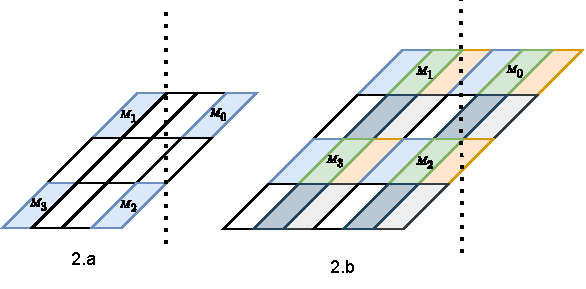
\includegraphics[width=\linewidth,scale=1.00]{fig2.pdf}    %[]里面的参数自己可根据需要调整
	\caption{Rectangular Karatsuba}
	\label{Figure2}
\end{figure}


\subsection{Barrett and Montgomery algorithm}
% \subsubsection{Algorithm process}
% \begin{figure}[htbp]   %单栏图片用{figure}; 双栏用{figure*},加个星号
% 	\centering
% 	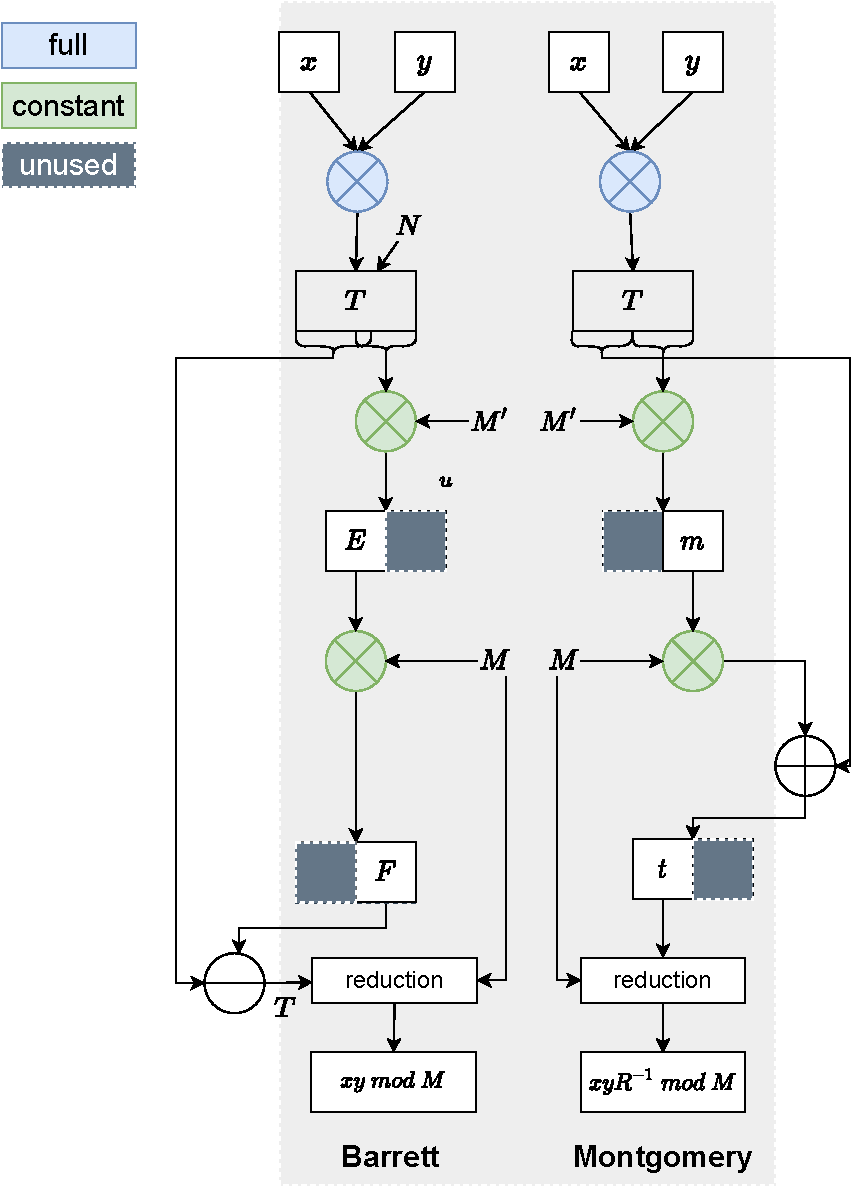
\includegraphics[width=\linewidth,scale=1.00]{fig3.pdf}    
% 	\caption{Barrett and Montgomery modular multiplication}
% 	\label{Figure3}
% \end{figure}

\textcolor{black}{
Barrett's algorithm and Montgomery are two of the most dominant algorithms for computing modular multiplications, which have similar structures, both consisting of three multiplications. The first one is a multiplication of two variables, and the latter two are multiplied by the modulus $M$ and a constant derived by $M$. 
}


The principle of Barrett algorithm can be simply summarized by calculating:
\begin{equation}
    E = \lfloor {{\lfloor {2^{2k}\over M} \rfloor {\lfloor {xy \over {2^{k-1}}}} \rfloor}\over 2^{k+1}} \rfloor \approx \lfloor xy / M\rfloor
\end{equation}
Then an estimate $E$ of $\lfloor N / M\rfloor$ is obtained. Immediately afterwards, by computing:
\begin{equation}
    T = xy-EM
\end{equation}
an estimate $T$ of $xy \% M$ is also obtained. It is obvious that $T \equiv xy\pmod{M}$. Finally, $xy \% M$ can be found by a single \textbf{fine reduction} ~\cite{Efficient_FPGA_Modular_Multiplication_Implementation} operation. For the original Barrett's algorithm, we have $T \in [0, YM)$, $Y \le 3$. So fine reduction can be done by at most two subtractions and MUX. From the principle, it can be found that the computation of $E$ is error-tolerant, and ~\cite{Efficient_FPGA_Modular_Multiplication_Implementation} shows that by discarding the LSBs part of the third multiplicative input, an error will be introduced to $E$, which increases $Y$ accordingly. However, within certain bounds, the correctness of the algorithm can be guaranteed by slightly increasing the complexity of the fine reduction, and the increase in complexity of the fine reduction is trivial compared to the decrease in multiplicative complexity in computing $E$.


\section{IMPLEMENTATION of the KARATSUBA MULTIPLIER}

\subsection{Variations of Multiplier Decomposition}    % 大数乘法器的分类学

\textcolor{black}{
Overall, long multipliers are achieved by the divide-and-conquer method, but according to the different targets, the split and merge operations have different implementations. Therefore, we divide them into 5 variations. For complete multiplication, there are two methods: Karatsuba and Schoolbook; For MSB multiplication, LSB multiplication, and square, there is one, respectively. Among them, MSB multiplication and LSB multiplication refer to the implementation discarding the lower or higher half input bits before calculation. They will be elaborated in the fifth part.
}

\textcolor{black}{
Figure \ref{Figure4} shows the five split and merge processes of the 2-split case, but they can all be generalized to the n-split case.
}


\begin{figure}[htbp]   %单栏图片用{figure}; 双栏用{figure*},加个星号
	\centering
	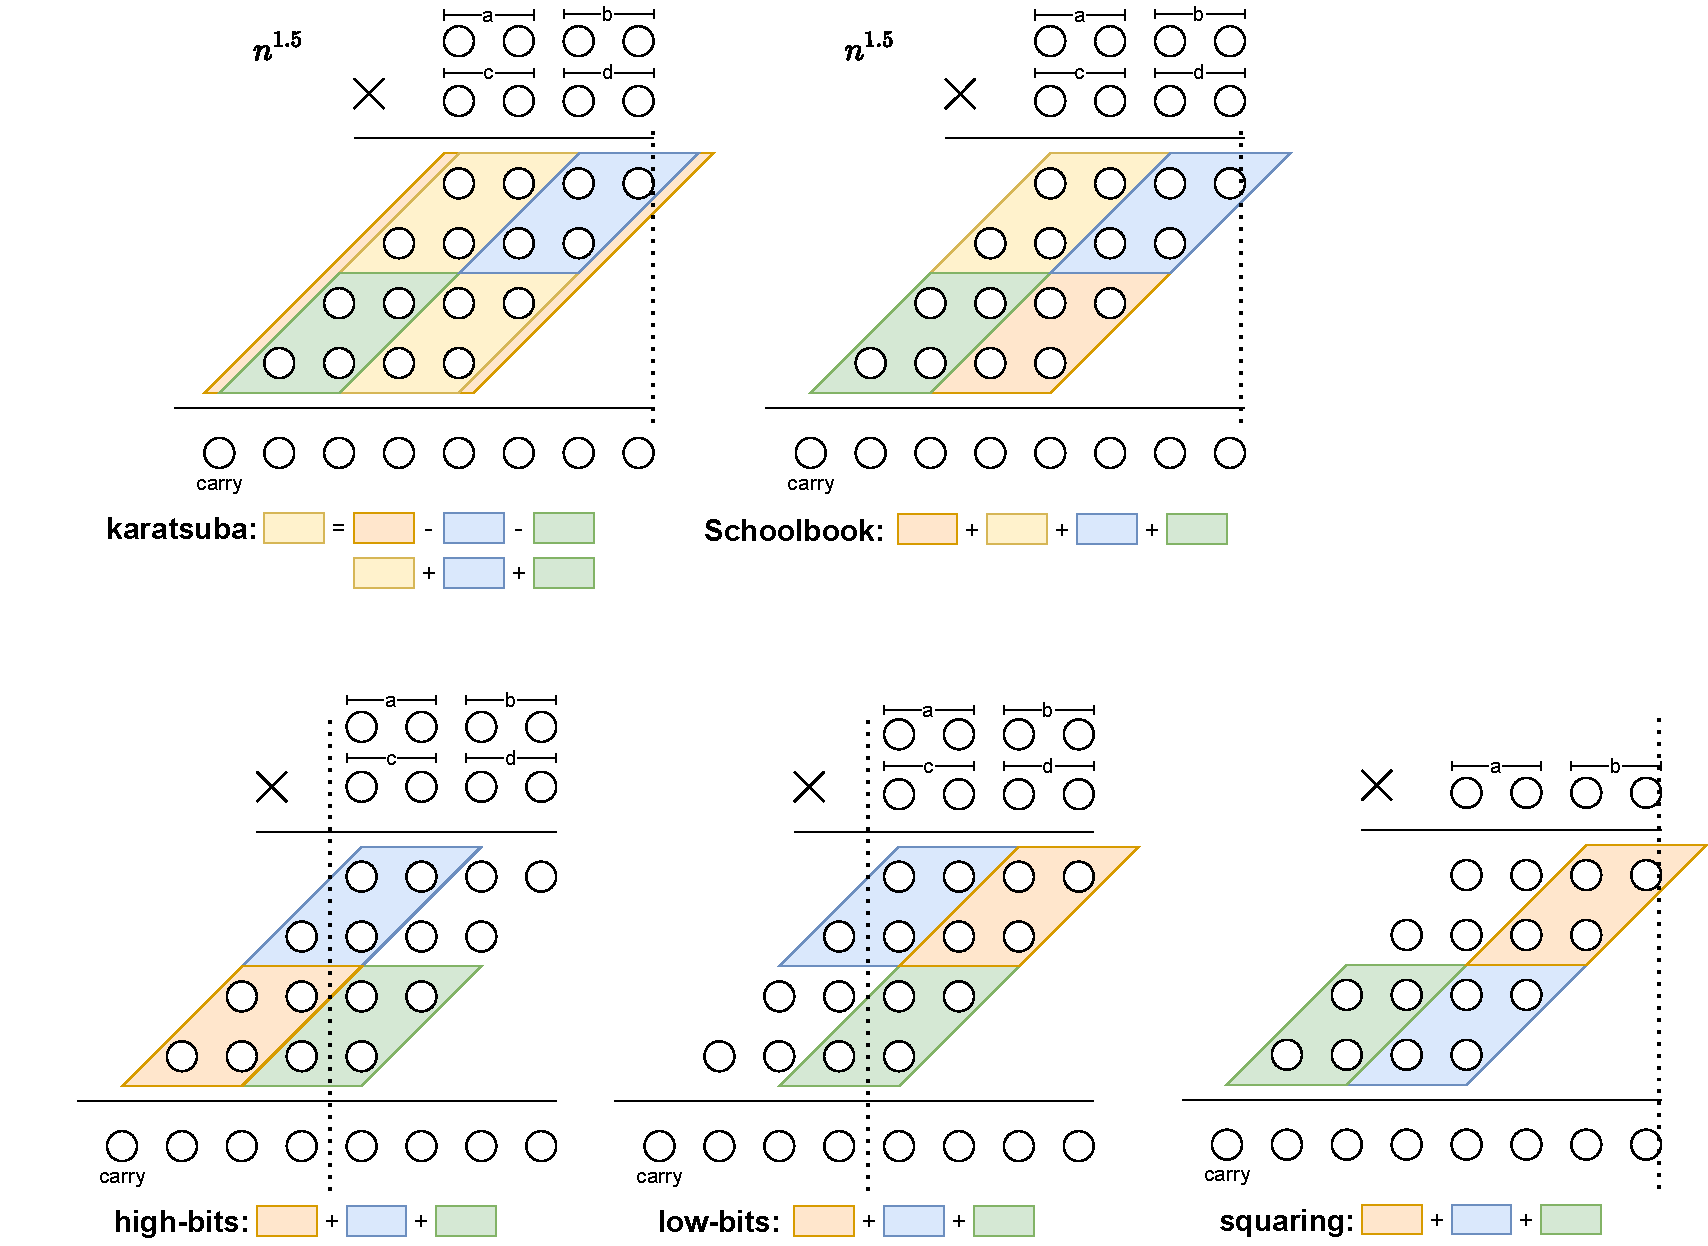
\includegraphics[width=\linewidth,scale=1.00]{fig4.pdf}    %[]里面的参数自己可根据需要调整
	\caption{Variations of split and merge}
	\label{Figure4}
\end{figure}


Let $A=a_12^W+a_0$, $B=b_12^W+b_0$, and we denote the complete multiplication result of $A,B$ as $f(A,B)$, the MSB,LSB,and square result as $m(A,B)$, $l(A,B)$, and $s(A,B)$. Formula 7 defines the implementations of each variation: 

\begin{equation}
    \begin{split}
    %\begin{alignedat}{1}
        f(A,B)&= f(a_1,b_1)2^{2W}+f(a_0,b_1)2^{W} \\
                & +f(a_1,b_0)2^{W}+f(a_0,b_0) \quad\quad\quad\quad { \text{Schoolbook}}\\
        f(A,B)&= f(a_1,b_1)2^{2W} \\
               & +(f(a_0+a_1,b_0+b_1)2^{W} - f(a_1,ab_0) - f(b_1, a_0)) \\
               & +f(a_0,b_0)  \quad\quad\quad\quad\quad\quad\quad\quad\quad\quad\quad  \text{Karatsuba}\\
       l(A,B) &= l(a_1,b_0)2^{W} + l(a_0,b_1)2^{W} + f(a_0,b_0)  \\
               & \quad\quad\quad\quad\quad\quad\quad\quad\quad\quad\quad\quad\quad\quad\quad\quad\quad\quad \text{LSB}\\
       m(A,B) &= m(a_1,b_1)2^{W} + m(a_0,b_1) + f(a_1,b_0)  \\
               & \quad\quad\quad\quad\quad\quad\quad\quad\quad\quad\quad\quad\quad\quad\quad\quad\quad\ \  \text{MSB}\\
       s(A,B) &= s(a_1,b_1)2^{W} + f(a_0,b_1)2^{W} + s(a_0,b_0) \\
               & \quad\quad\quad\quad\quad\quad\quad\quad\quad\quad\quad\quad\quad\quad\quad\quad \text{SQUARE}\\
    %\end{alignedat}
    \end{split} 
\end{equation}

\textcolor{black}{
Based on this, we can define a \textbf{decomposition} as the basic unit of the implementation of a long multiplier, where a decomposition is a 4-tuple:
\begin{equation}
    ((h,w), n, \text{multType}, \text{isKara} )
\end{equation}
This 4-tuple uniquely portrays a decomposition, and the options available for a decomposition include:
\begin{itemize}
    \item dsp size $(h,w)$. For the last layer of decomposition, the size can be rectangular to fit the embedded multiplier size on modern FPGAs. For other layer, the size is a square size, where $h = w$.
    \item $n$, which is the number of split.
    \item $\text{multType} = \{\text{FULL} |\text{MSB}|\text{LSB}|\text{SQUARE}\}$. The objective of the solution include complete multiplication, MSB multiplication, LSB multiplication and square.
    \item $\text{isKara} = \{0|1\}$. For complete multiplication, this property defines whether the decomposition is Karatsuba or Schoolbook.
\end{itemize}
}

\subsection{Karatsuba Sub-Components on FPGAs}    % 大数乘法器组成部分

\textcolor{black}{
On the pipelined large multiplier, the split-multiplication-merge structure can be mapped into a three-stage structure, as shown in Figures \ref{Figure5}. We refer to these three parts as: 
\begin{itemize}
    \item Pre-addition tree, which consists of addition and split.
    \item Multiplication line, which consists of multiplication and MUX(multiplication with a 1-bit operand), where multiplication dominates.
    \item Post-additive network, which consists of addition and shifting.
\end{itemize}
}

\begin{figure}[htbp]   %单栏图片用{figure}; 双栏用{figure*},加个星号
	\centering
	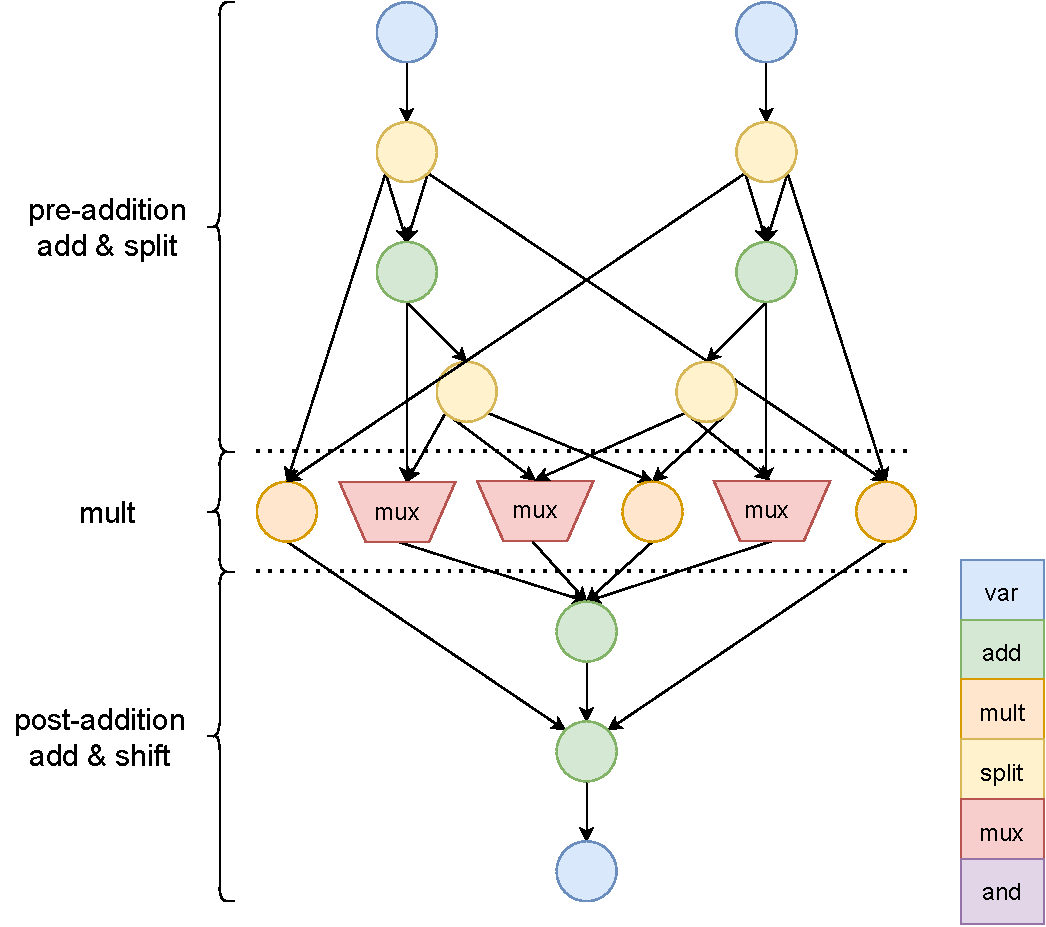
\includegraphics[width=\linewidth,scale=1.00]{fig5.pdf}    %[]里面的参数自己可根据需要调整
	\caption{Three-stage implementation of long multiplier}
	\label{Figure5}
\end{figure}


\textcolor{black}{
Figure \ref{Figure5} is the case of $2$-split Karatsuba decomposition. In order to deal with the increase of the width of the cross-term, we separate the MSB of the cross-term, which brings the three multiplex operations.}
\textcolor{black}{
According to their implementations on FPGA, these three parts correspond to four types of units: (long) binary carry adders (CPA), embedded multipliers, compressor tree (i.e. carry-save adder (CSA)), and two-input multiplexer. Among them, the common feature of the first three types of units is that they perform merge arithmetic, and the purpose of merge arithmetic is to "eliminate bits", so the "performance" of these three types of units can be measured through the same scale, i.e., the number of bits eliminated. In fact, not only on Karatsuba multipliers, but all computational units in the entire modular multiplier can be classified into these three categories, except for the mux operations in the fine reduction part and the Karatsuba cross-term carry processing part. On the FPGA architecture, the LUT area overhead of a two-input MUX is equivalent to a two-input carry multiplication with the same width. Therefore, we also include it as the CPA consumption in the subsequent calculations.
}


\subsubsection{Analysis of Pre-Additive Trees}    % 前加法树的分析

\textcolor{black}{
The task of the pre-additive tree is to divide the inputs into segments that can be fed into the basic multiplier. Addition exists in the pre-addition tree when Karatsuba decomposition is included in the architecture. In fact, there are two identical pre-addition trees in the hardware architecture of Karatsuba and each tree depends on only one multiplicand. When the goal is to achieve constant multiplication instead of full multiplication, all nodes on one of the trees can be determined at compile time, and accordingly, all multiplications on the multiplication line become constant multiplications.
}

\subsubsection{Analysis of Post-Additive Networks}    % 后加法网络的分析

The use of compressor tree is also mentioned in the work of ~\cite{Heuristics_for_the_Design_of_Large_Multipliers_for_FPGAs}, but no in-depth analysis has been performed, while in most of other works, compressor tree is not used. The implementation of Karatsuba post-additive network using compressor tree has at least the following benefits:
\begin{enumerate}[(1)]
    \item Avoid pipeline and critical path bottlenecks caused by long CPAs. Collectively, the additive widths in the post-additive network are larger than in that the pre-additive tree, generally reaching twice the size of the pre-additive tree (because the output of multiplication is twice that of addition). By using rounding-preserving addition, long rounding additions can be completely avoided during the computation, and the length of the rounding chain is limited only by the length of the basic compressor.
    \item The use of compressor tree also avoids the latency expansion associated with the padding of aligned pipeline for large bit-width carry look-ahead adder.
    \item In general, on modern FPGAs, with the help of the three-input adder and 4-2 compressor, the area efficiency of the compressor tree can theoretically approach twice that of the two-input adder when the input size is large enough. In practice, on a small-sized compressor tree, its efficiency is slightly better than that of a two-input adder; on a large-sized compressor tree, the area efficiency can reach 1.7 $\sim$  1.8 times of the two-input adder. There is a discussion on this conclusion in ~\cite{Karatsuba_with_Rectangular_Multipliers_for_FPGAs}, which is also verified in our cost model and experiments.
\end{enumerate}

\textcolor{black}{
We did further analysis of Karatsuba's compressor tree. It should be noted that when we describe the three components, we use the phrase "post-addition \textbf{network}" instead of "tree". This is because the combined part in the Karatsuba decomposition is not completely tree-like. The product terms on the diagonal (Figure \ref{Figure1}) are reused when using the Karatsuba decomposition.
}

\textcolor{black}{
In this scenario, if the entire addition network is implemented as a multi-input addition, all nodes before the multiplexed node will contribute to the bit heap multiple times, which actually increases the computational complexity (that is, the number of the bits needed to be eliminated). Taking Figure \ref{Figure6} as an example, if a partial result is obtained at node B, then node A is only eliminated twice; but if the entire addition network is to be implemented as a multi-input addition, then node A needs to be eliminated four times since there are 4 paths from node A to node C.
}


\begin{figure}[!htb]    % 双栏图
	\centering  %图片全局居中
	\subfigbottomskip=2pt  %两行子图之间的行间距
	\subfigcapskip=-5pt  %设置子图与子标题之间的距离
	\subfigure[4 paths of the sam operand.]{
		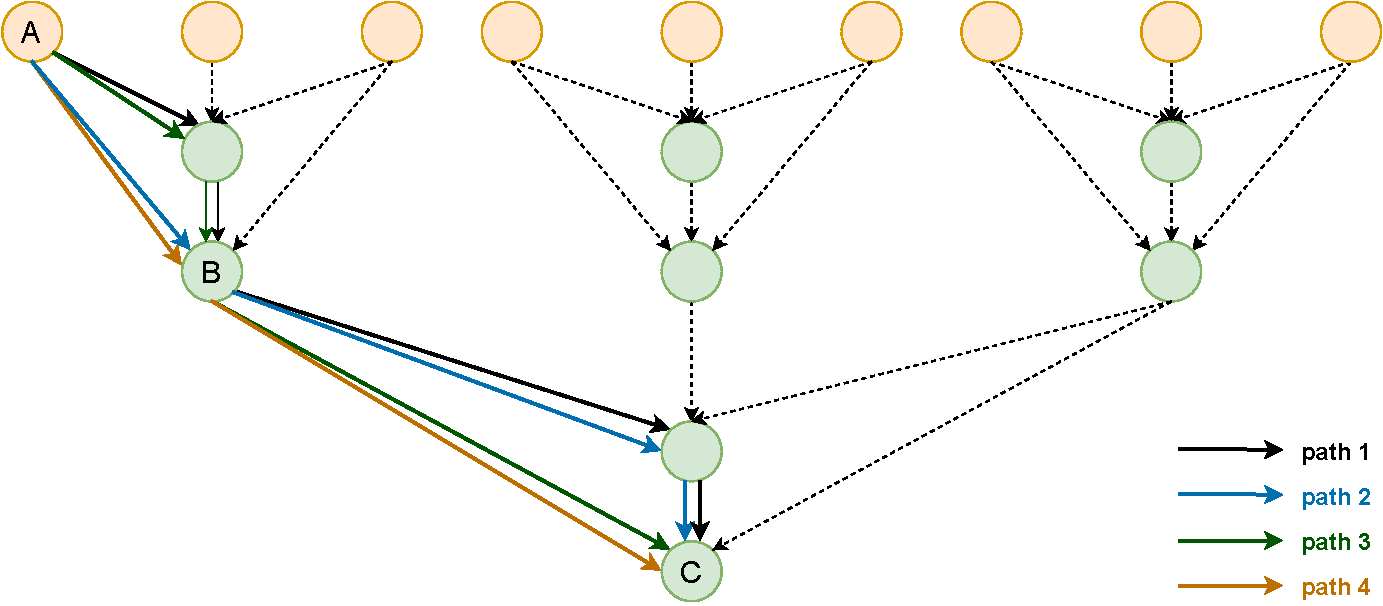
\includegraphics[width=0.48\linewidth]{fig6a.pdf}}
	\subfigure[Trees after rewriting, the main(green) tree and the others.]{
		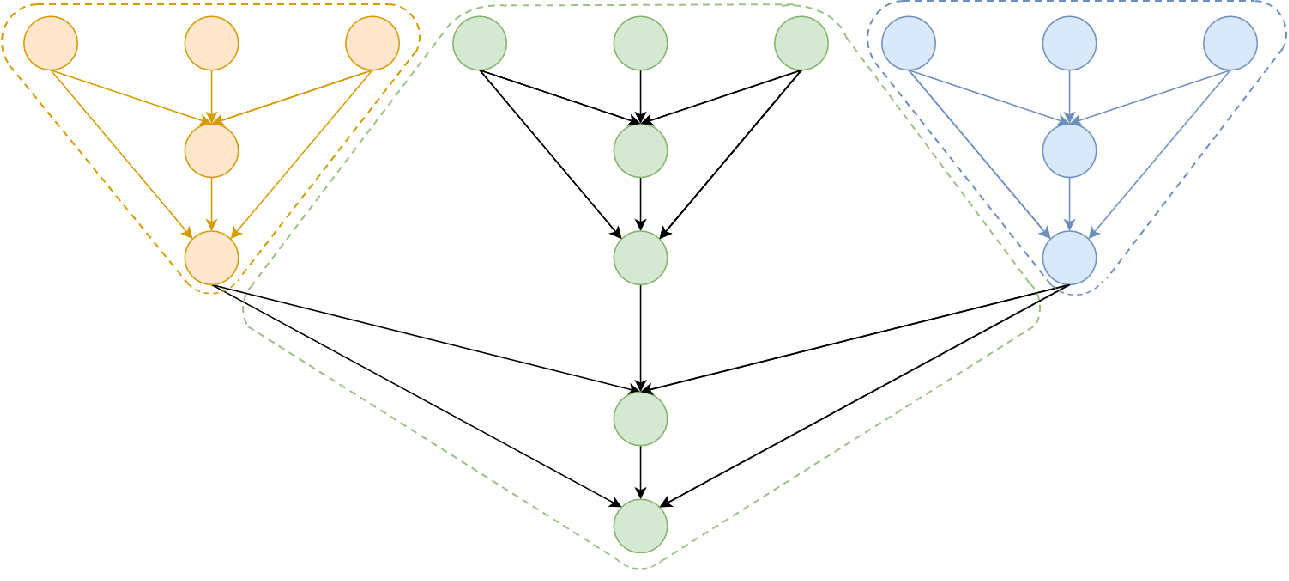
\includegraphics[width=0.48\linewidth]{fig6b.pdf}}
	\caption{}
	\label{Figure6}
\end{figure}


\textcolor{black}{
In our implementation, the backward addition network is divided into a master tree and several slave trees. Our generator extract and implement the trees in the backward addition network using the fan-out as the judgment criterion. Since the bit heap data structure supports the time difference input ~\cite{Arithmetic_core_generation_using_bit_heaps}, the start of the master tree computation does not need to wait for the completion of the slave tree computation. Through this method, we merge small compressor trees into a large compressor tree as much as possible to improve the compression efficiency.
}

\subsection{Primitive Level Implementation of Long Multipliers}    % 大数乘法器的原语级实现

\textcolor{black}{
For the three components mentioned above, we have carried out primitive level optimization for FPGA implementation, more specifically:
\begin{itemize}
  \item For long carry-propagation adders, in addition to the most common binary(2-input) addition/subtraction, we also implement the ternary adder with three modes of ($a+b+c$, $a+b-c$, $a-b-c$) through the LUT6\_2 primitive and the CARRY8 primitive. When splitting a long carry-propagation carry adder into different pipeline stages, our algorithm matches the segment size to the multiple of CARRY8 size to utilize CARRY8 as efficiently as possible.
    \item For compressor trees, GPCs and row-adders~\cite{Arithmetic_core_generation_using_bit_heaps} are implemented directly by LUT6\_2 and CARRY8 primitives to get the best LUT efficiency.
    \item For embedded multipliers, we conduct dedicated DSP datapath optimizations that serve two purposes:
    \begin{enumerate}[(1)]
        \item To precisely control the synthesizer's mapping and pipeline strategy for DSP to avoid unexpected critical path increments.
        \item Efficiently utilizes computing resources other than embedded multipliers in the DSP slice of modern FPGAs to reduce area overhead. Specifically, taking Xilinx's DSP48E2 DSP ~\cite{UltraScale_Architecture_DSP_Slice_User_Guide} as an example, in addition to one embedded multiplier, it also has a pre-adder and an ALU (which can perform an addition/subtraction) inside. However, utilizing these resources accurately through the general RTL description and synthesizer inference is difficult. Therefore, in implementing the long multiplier, we designed dedicated DSP datapaths for three variations to reduce area overhead.
    \end{enumerate}
\end{itemize}
}

\textcolor{black}{
As shown in Table \ref{Naive_Refined}, the primitive-based implementation faithfully produces the pipeline we expected, with significant area advantages over the implementation obtained by RTL description + synthesizer retiming. 
}

\begin{table}[ht]
    \centering
    \caption{Comparison of Resource Usage between Naive and Refined Realization of Different Multipliers.}
    \renewcommand{\arraystretch}{1.1}
    \begin{tabular}{l|c|c|c|c|c}
        \Xhline{1.5pt}
        % \specialrule{0em}{0pt}{2pt}    % 为什么会断开呢?
                                      & Realization & LUT6 &  FF  & DSP & CARRY8 \\  
        \Xhline{1pt}
        \multirow{2}{*}{Karabase}     &    Naive    &  113 &  136 &  4  &   3    \\
        \cline{2-6}
                                      &   Refined   &  49  &  87  &  3  &   8    \\
        \Xhline{1pt}
        \multirow{2}{*}{Full-Mult}    &    Naive    &  120 &  122 &  5  &   10   \\
        \cline{2-6}
                                      &   Refined   &  115 &  266 &  3  &   15   \\
        \Xhline{1pt}
        \multirow{2}{*}{Square-Mult}  &    Naive    &  73  &  122 &  5  &   7    \\
        \cline{2-6}
                                      &   Refined   &  68  &  121 &  3  &   6    \\
        \Xhline{1.5pt}
    \end{tabular}
    \label{Naive_Refined}
\end{table}

\subsection{Cost Model of Long Multipliers}    % 大数乘法器代价模型

\textcolor{black}{
With the bit heap theory, taxonomy and primitive-level implementation that mentioned above, we can build an accurate cost model for the implementation of Long multipliers on FPGA.
Firstly, we provide the cost of different computational primitives in Table  \ref{computational_primitives_cost}. $h$ and $w$ are the height and the width of an embedded multiplier, $w_i$ are input widths of compressor tree while $w_o$ is the output width.
}

\begin{table}[ht]
    \centering
    \caption{Cost In DSP And LUT Of Different Components}
    \renewcommand{\arraystretch}{1.5}
    \begin{tabular}{l|c|c|c}
                \Xhline{1.5pt}
                         & \makecell[c]{numbers of \\ bits reduction} & DSP  & LUT      \\
                \Xhline{1pt}
        embedded multiplier     &   $ hw-h-1 $  &   $1$ &   $0$    \\
                \Xhline{1pt} 
        binary adder   &   $ w-1 $     &   $0$ &   $w$    \\
                \Xhline{1pt}
        ternary adder  &   $2(w-1)$    &   $0$ &   $w$    \\
                \Xhline{1pt} 
        compressor tree  &  $ \sum_{i=1}^n w_i-w_o $    &   $ 0 $   &   reduction/efficiency    \\
                \Xhline{1.5pt} 
    \end{tabular}
    \label{computational_primitives_cost}
\end{table}

\textcolor{black}{
A cost model for Karatsuba decomposition can be obtained by summing the cost of components. We take the 4-tuple $((h,w), n, \text{FULL}, 1)$ as an example for analysis (Figure \ref{Figure5}). In this decomposition, there are $n$ sub-multipliers on the diagonal and $n(n-1)\over 2$ basic Karatsuba computations.
\begin{itemize}
    \item Each basic Karatsuba computations brings two CPAs, totaling ${n(n-1)\over 2}(h+w)$.
    \item The merge cost is the cost of summing all multiplication results through the compressor tree. For a sub-multiplier on the diagonal, this includes only a product with a width of $h+w$. For a basic Karatsuba calculation, the three products used to generate the cross terms and the three MUX results are included, with a combined width of $3(h+w)+(h+w+1) = 4(h+w)+1$ and a total cost of ${n(n-1)\over 2}[4(h+w)+1] + n(h+2)$. It should be noted that the previously mentioned combination of compressor trees in the post-addition network does not change the cost.
    \item The multiplication cost consists of two parts, the first part is the MUX cost that takes effect immediately, and the other part is the embedded multiplier cost that takes effect on the last level of decomposition. The implementation cost of the two-input MUX is comparable to that of the two-input adder, totaling ${n(n-1)\over 2}(h+w+1)$. Before the last level of decomposition, the multiplication cost is cached as the number of sub-multipliers, which is $n(n+1)\over 2$, and the actual cost is incurred only at the last level of decomposition.
\end{itemize}
}

\textcolor{black}{
With the same analysis method, we can obtain the cost model of all variants, and the costs of all variants are listed in the table \ref{cost}.
}

\begin{table*}[ht]
    \centering
    \caption{Primitive cost of variations of multiplication}
    \renewcommand{\arraystretch}{1.1}
    \begin{tabular}{l|c|c|c|c}
                \Xhline{1.5pt}
                        & split cost & merge cost & mux cost & sub-multiplier \\
                \Xhline{1pt}
        full-schoolbook &   0         & $n^2(h+w) - w_o$ &  0         &    $n^2$       \\
                \Xhline{1pt}
        full-Karatsuba  &   ${n(n-1)\over 2}(h+w)$        &     ${n(n-1)\over 2}[4(h+w)+1] + n(h+2) - w_o $       &    $h+w+1$       &     ${n(n+1)\over 2}$      \\
                \Xhline{1pt}
        square          &    0        &     $3(h+w) - w_o $       &   0        &     ${n(n+1)\over 2}$      \\
                \Xhline{1.5pt}    
    \end{tabular}
    \label{cost}
\end{table*}

\textcolor{black}{
Further, we obtain the cost model of the complete large-number multiplier scheme. A complete large-number multiplier scheme is a tree composed of multiple decompositions, and its LUT cost is the sum of the LUT cost in each decomposition:
\begin{equation}
    C_{\text{LUT}}(\text{solution}) = \sum_{n\in \text{nodes}}C_{\text{LUT}}(n)
\end{equation}
The DSP cost is the sum of the cumulative multiplications of all sub-multipliers from the root to the leaf nodes:
\begin{equation}
    C_{\text{DSP}}(\text{solution}) = \sum_{n\in \text{leaves}}\prod _{m \in \text{path to n}}C_{\text{DSP}}(m)
\end{equation}
}


\begin{figure}[htb]   %单栏图片用{figure}; 双栏用{figure*},加个星号
	\centering
	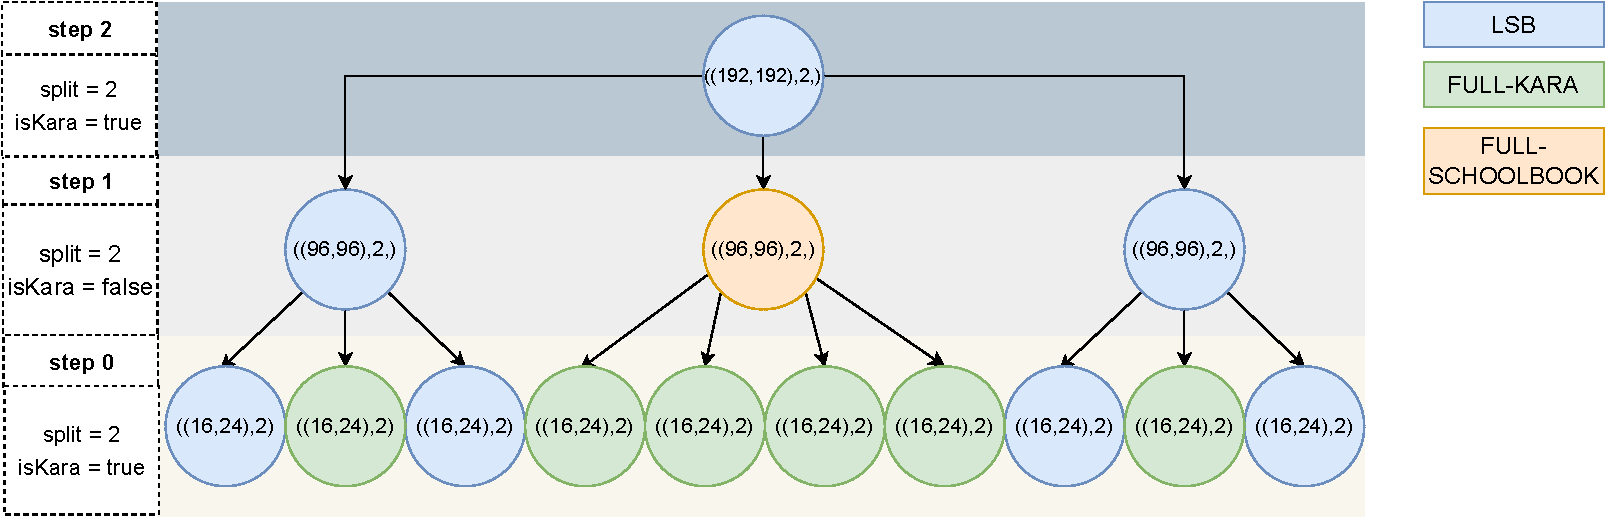
\includegraphics[width=\linewidth,scale=1.00]{fig8.pdf}    %[]里面的参数自己可根据需要调整
	\caption{Decision tree of building a long multiplier.}
	\label{Figure8}
\end{figure}


\subsection{Searching for Karatsuba Architecture Schemes}    % 架构搜索算法
\begin{algorithm}[ht]
    \caption{Architecture Search Algorithm} %算法名字
    \label{alg2}
	\LinesNumbered %要求显示行号
    \KwIn{Effective dsp size set $dsps$, target width $W$, target multiplier type $mult$} %输入参数
	\KwOut{The Pareto-optimal solution set $solutionSet$ that achieves the target width} %输出参数
    init solutionSet \;
    \For{$dsp$ in $dsps$}{
        $solutionSet \mathrel{+}= solution(dsp, 2, mult, true)$ \;
    }
    \While{undeterminedOf(solutionSet) is not empty}{
        $solutionsOld = undeterminedOf(solutionSet)$ \;
        \For{$solution$ in $undeterminedOf(solutionSet)$}{
            $split = 2$ \;
            \While{$(widthOf(solutionNext)) < W)$}{
                $solutionNext0 = expand(solution, split, true)$ \;
                $solutionNext1 = expand(solution, split, false)$ \;
                $solutionSet \mathrel{+}= solutionNext0$ \;
                $solutionSet \mathrel{+}= solutionNext1$ \;
                $split \mathrel{+}= 1	$ \;
            }
            repeat $11-14$ \;
        }
        $makePareto(solutionSet)$ \;
        $solutionSet \mathrel{-}= solutionsOld$ \;
    }
    $makePareto(solutionSet)$ \;
\end{algorithm}


\textcolor{black}{
A complete \textbf{architecture scheme} of a large multiplier contains multiple decompositions in a tree-like structure, as shown in the Figure \ref{Figure8}. In our strategy, the architecture search is performed layer by layer, and all combinations at each layer of the tree use the same $\text{isKara}$ And split properties. Because starting from the target width, after the first decomposition, the obtained sub-problems have same size, and the optimal decomposition strategy should also be the same. Therefore, the large-number multiplier architecture scheme can be fully defined by a 4-tuple:
\begin{equation}
    ((h,w), (n_1 \cdots n_{k}), \text{multType}, (\text{isKara}_1 \cdots \text{isKara}_k))
\end{equation}
In which:
\begin{itemize}
    \item $h,w$ is the DSP size of the last level.
    \item $n_i$ is the split for each level.
    \item $\text{multType} $ specifies the target of the entire multiplier implementation.
    \item $\text{isKaras}_i$ specifies whether the full multiplication in each layer is implemented using the Karatsuba decomposition.
\end{itemize}
}


\textcolor{black}{
An example is given in Figure \ref{Figure8} which is denoted as $((16,24), (2,2,2), \text{LOW}, (1,0,1))$.
}


\textcolor{black}{
Since there are different resources on the FPGA, we firstly define a unified optimization objective to avoid dealing with multi-objective optimization problems. A more reasonable strategy is setting the number of operators implemented as the unified objective. In actual tasks, usually we have a fixed FPGA budget, our goal is to achieve as many pipelined operators as possible under the constraints of this budget and then hand over these operators to the control logic for scheduling. Such design paradigm has been widely adopted in related works such as ~\cite{PipeMSM} 
~\cite{FPGA_Acceleration_of_Multi_Scalar_Multiplication_CycloneMSM}. This problem is essentially an integer linear programming problem, which is defined as follows:
}


\textcolor{black}{
Input: An FPGA resource budge $(\text{LUT}_{\text{all}}, \text{DSP}_{\text{all}}) $, and a set of solutions $(\text{LUT}_1, \text{DSP}_1) \cdots (\text{LUT}_k, \text{DSP}_k) $.
}

\textcolor{black}{
Target: Numbers of each solution $s_1 \cdots s_k$.
}


Constraint:
\begin{equation}
    \sum s_i \text{LUT}_i \le \text{LUT}_{\text{all}} \ , \ \sum s_i \text{DSP}_i \le \text{DSP}_{\text{all}} 
\end{equation}


Goal:
\begin{equation}
    \operatorname{maximize}(\sum s_i )
\end{equation}


\textcolor{black}{
We propose a long multiplier architecture search algorithm based on branch-and-bound and dynamic programming to produce the Pareto optimal solutions required for the problem above. Because the algorithm searches through a tree, and it satisfies the optimal substructure property. That is, a sub-solution of the Pareto optimal solution must also be optimal at its size. In this algorithm, we search from the DSP size, in a bottom-up manner. Our algorithm searches from several pre-specified efficient DSP sizes (lines 3-5 of code) in a branching delimitation method. Specifically, at each search step, we branch (lines 10-17) by traversing possible splits and $\text{ isKara }$ for each solution that has not yet reached the target width (obtained by the \textbf {undeterminedOf }function) until the width exceeds the target width. After each iteration, we classify all solutions in the solution set according to their current width, leaving only the Pareto optimal solutions on each class, pruning (line 19), and discarding the branched solution (line 20). We repeat this process until the solution set no longer contains solutions that have not reached the target width. Finally, we retain all Pareto optimal solutions on the solution set (line 22).
}

\textcolor{black}{
For the first decomposition from the bottom up, the algorithm has a special treatment (line 4). Only on this layer, we allow the rectangular size and specify $n_1 = 2, text{isKara}_1 = 1$, because on this decomposition, we can make good use of the dedicated routing resources and additive computing resources of the DSP itself to handle the additional overhead of Karatsuba decomposition. Moreover, the DSP size of the FPGA itself may be rectangular.
}

% \section{MODULAR MULTIPLIER IMPLEMENTATION}
% \subsection{Big Constant Multiplier as Compressor Tree}
% \subsection{Barrett Reduction with Bits Dropped}
% \subsection{Improved Fine Reduction Module}

\section{BARRETT MULTIPLIER IMPLEMENTATION}

\subsection{Taxonomy of Modular Multipliers}

\begin{figure}[htbp]   %单栏图片用{figure}; 双栏用{figure*},加个星号
	\centering
	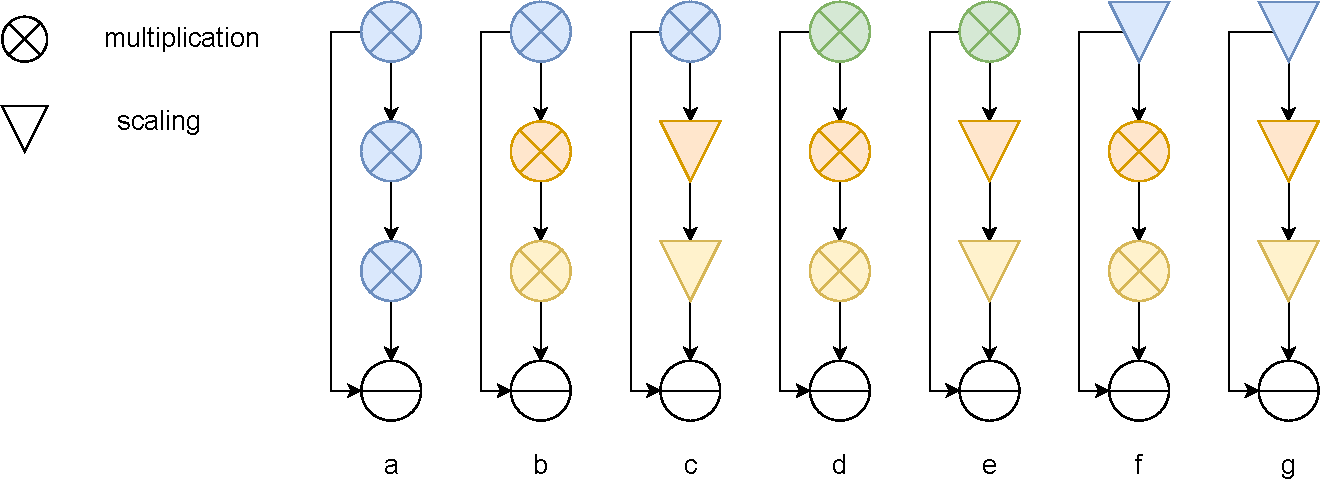
\includegraphics[width=\linewidth,scale=1.00]{fig9.pdf}    %[]里面的参数自己可根据需要调整
	\caption{Variations of modular multipliers.}
	\label{Figure9}
\end{figure}

As with many large number multipliers,  we improve the level of customization for the modular multiplier by classifying the implementation of it to obtain area gains. In the case of using the Barrett/Montgomery algorithm, at least the following variants exist:
\begin{itemize}
    \item Modular multiplication/modular squaring, which affects the way the first multiplier is implemented.
    \item Modular multiplication of variables with variables/constants, influencing whether the first multiplier in Montgomery/Barrett can be implemented as a constant multiplier.
    \item Modular-fixed/modular-variable modular multiplication, which has an impact on whether the second and third multipliers in Montgomery/Barrett can be implemented as constant multipliers.
\end{itemize}

All these variations can be implemented the most general ways, i.e. modular multiplication of variables, which corresponds to Figure \ref{Figure9}. This is how most area and power oriented work has been implemented in the past.  However, implementations of other variants on FPGAs are becoming more and more profitable for two reasons:
\begin{enumerate}[(1)]
    \item As modern FPGAs have more and more resources, the size of the arithmetic that can be unfolded on FPGAs has increased. The richness of elliptic curve algorithms makes it possible for all of the cases listed above to occur in a high-throughput implementation. For instances, ~\cite{FPGA_Acceleration_of_Multi_Scalar_Multiplication_CycloneMSM} utilizes an algorithm on twisted edwards curves that includes a modular multiplication with large constants, and ~\cite{PipeMSM} exploits a montgomery ladder algorithm that includes four modular square multiplication.
    \item As FPGAs become more widely used in data centers and move towards clustering and virtualization, algorithms that would otherwise require variable/multiple modules may also be supported by multiple FPGAs, or multiple reconfigurable regions on a single FPGA, through clustering, or partial reconfigurability
\end{enumerate}

When the degree of expansion is greater than single modular multiplier (e.g., up to an additive unit on an elliptic curve, which may include modular multipliers, modular squares and constant modular multipliers),  then the implementations of Figures \ref{Figure9}.d-\ref{Figure9}.g may become the best implementations, a degree of expansion that is not uncommon in today's applications. This degree of expansion is achieved in ~\cite{FPGA_Acceleration_of_Multi_Scalar_Multiplication_CycloneMSM}. Therefore, a hardware generator that can generate all the following variants can greatly improve the hardware efficiency of the modular multiplier in a highly expanded system.

To implement such a generator, we need to implement an efficient long constant multipliers generator and extend the truncated version of Barrett modular multiplicationin ~\cite{Efficient_FPGA_Modular_Multiplication_Implementation} to work with CSD encoding. These are given in the following sections.

\subsection{Implementation of Large Constant Multiplier}

\subsubsection{Analysis}

\textcolor{black}{
We have adopted the LUT+compression tree based approach for the implementation of the large constant multiplier instead of the DSP+partitioning approach, due to comparative advantages of the CLB resources and the compression tree approach for the implementation of the constant multiplier.
}

We first analyze the cost of implementing constant multiplication using a compressor tree. A constant multiplier of size $h\times w$ and constant width $w$, with $w$ sufficiently large, we can assume that the number of non-zero bits is $w\over 2$, so the overhead of this compressor tree is ${{hw} \over 2} - h - w$.

Further, we represent the constants in CSD encoding, statistically, CSD encoding can further reduce $1\over 3$ non-zero bits compared to binary encoding, and the overhead is reduced to ${{hw} \over 3} - h - w$.

\textcolor{black}{
In fact, in many cryptographic algorithms, the modulus is not randomly obtained,  but often sparse, e.g., the 377-bit modulus of the BLS12-377 curve in zkSNARK has only 135 non-zero bits in binary form and 98 non-zero bits in CSD form.
}

\textcolor{black}{
In the following, we discuss the advantages and disadvantages of  three constant multiplier implementations for a scenario where the target width is $H \times W$ and the basic multiplier width is $h \times w$.
\begin{enumerate}[(1)]
    \item Partitioning + DSP.
    \item Partitioning + LUT.
    \item Complete compression tree + LUT.
\end{enumerate}
}

\textcolor{black}{
Scheme 1 is the constant version of the large multiplier scheme in Section 3.  The splitting overhead of the constant multiplier will be halved,  but the multiplier overhead and merge overhead will remain the same for the DSP and partitioning based large number multiplication implementations.  This means that in the DSP part, there is no gain from constants, and in the LUT part, the gain from constants does not exceed 12.5\%,  because there is no split overhead when Karatsuba decomposition is not used. When Karatsuba decomposition is used, the overhead share of the overall LUT overhead does not exceed its share in one basic Karatsuba operation,  i.e. ${(h+w)\over {4(h+w)+1}} \ge 25\%$
}

\textcolor{black}{
In Scheme 2, we follow the partitioning method in the large number multiplier scheme. However, the multiplication part, which was originally implemented by DSP, is implemented by compressing the tree instead. Thus, for the same solution, the DSP overhead is zeroed and the LUT overhead is increased from $C_{\text{LUT}}$ to
\begin{equation}
    C_{\text{LUT}} + {C_{\text{DSP}}(hw-h-w)\over 3\text{eff}}
\end{equation}
}

% \textcolor{black}{
In Scheme 3, we treat the entire constant multiplier as one and implement it through a compressor tree, which has an overhead of:
\begin{equation}
    HW - H - W \over {3\text{eff}}
\end{equation}
% }

% \textcolor{black}{
However, in the context of modular multiplication,  this implementation also has a constant factor gain from the MSB/LSB multiplication, which is about 50\%, with a real overhead of about
\begin{equation}
    HW - H - W \over {6\text{eff}}
\end{equation}
% }

\textcolor{black}{
Overall, the asymptotic complexity is sub-quadraic on both DSP and LUT due to the use of scheme 2.  As the width increases, the overhead of Scheme 2 will finally be smaller than that of Scheme 3. However, in practice, Scheme 2 has some other drawbacks including:
\begin{enumerate}[(1)]
    \item A larger constant factor is required.
    \item A rather complex pipeline and the corresponding cost on padding for aligned pipeline are caused by multi-layer nesting.
    \item It brings multiple small-scale, rather than a single large-scale compressor tree, on which cells, $\text{eff}$ is worse.
    \item The divide and conquer approach is less exploitative for MSB/LSB scenarios.
\end{enumerate}
}

\textcolor{black}{
From the experimental results, the overhead of Scheme 2 starts to be lower than that of Scheme 3 when the width reaches nearly 8192 for MSB/LSB multiplication, so we adopt Scheme 3 as our large width constant multiplier scheme.
}

\subsubsection{Implementation}


% \begin{figure}[htbp]   %单栏图片用{figure}; 双栏用{figure*},加个星号
% 	\centering
% 	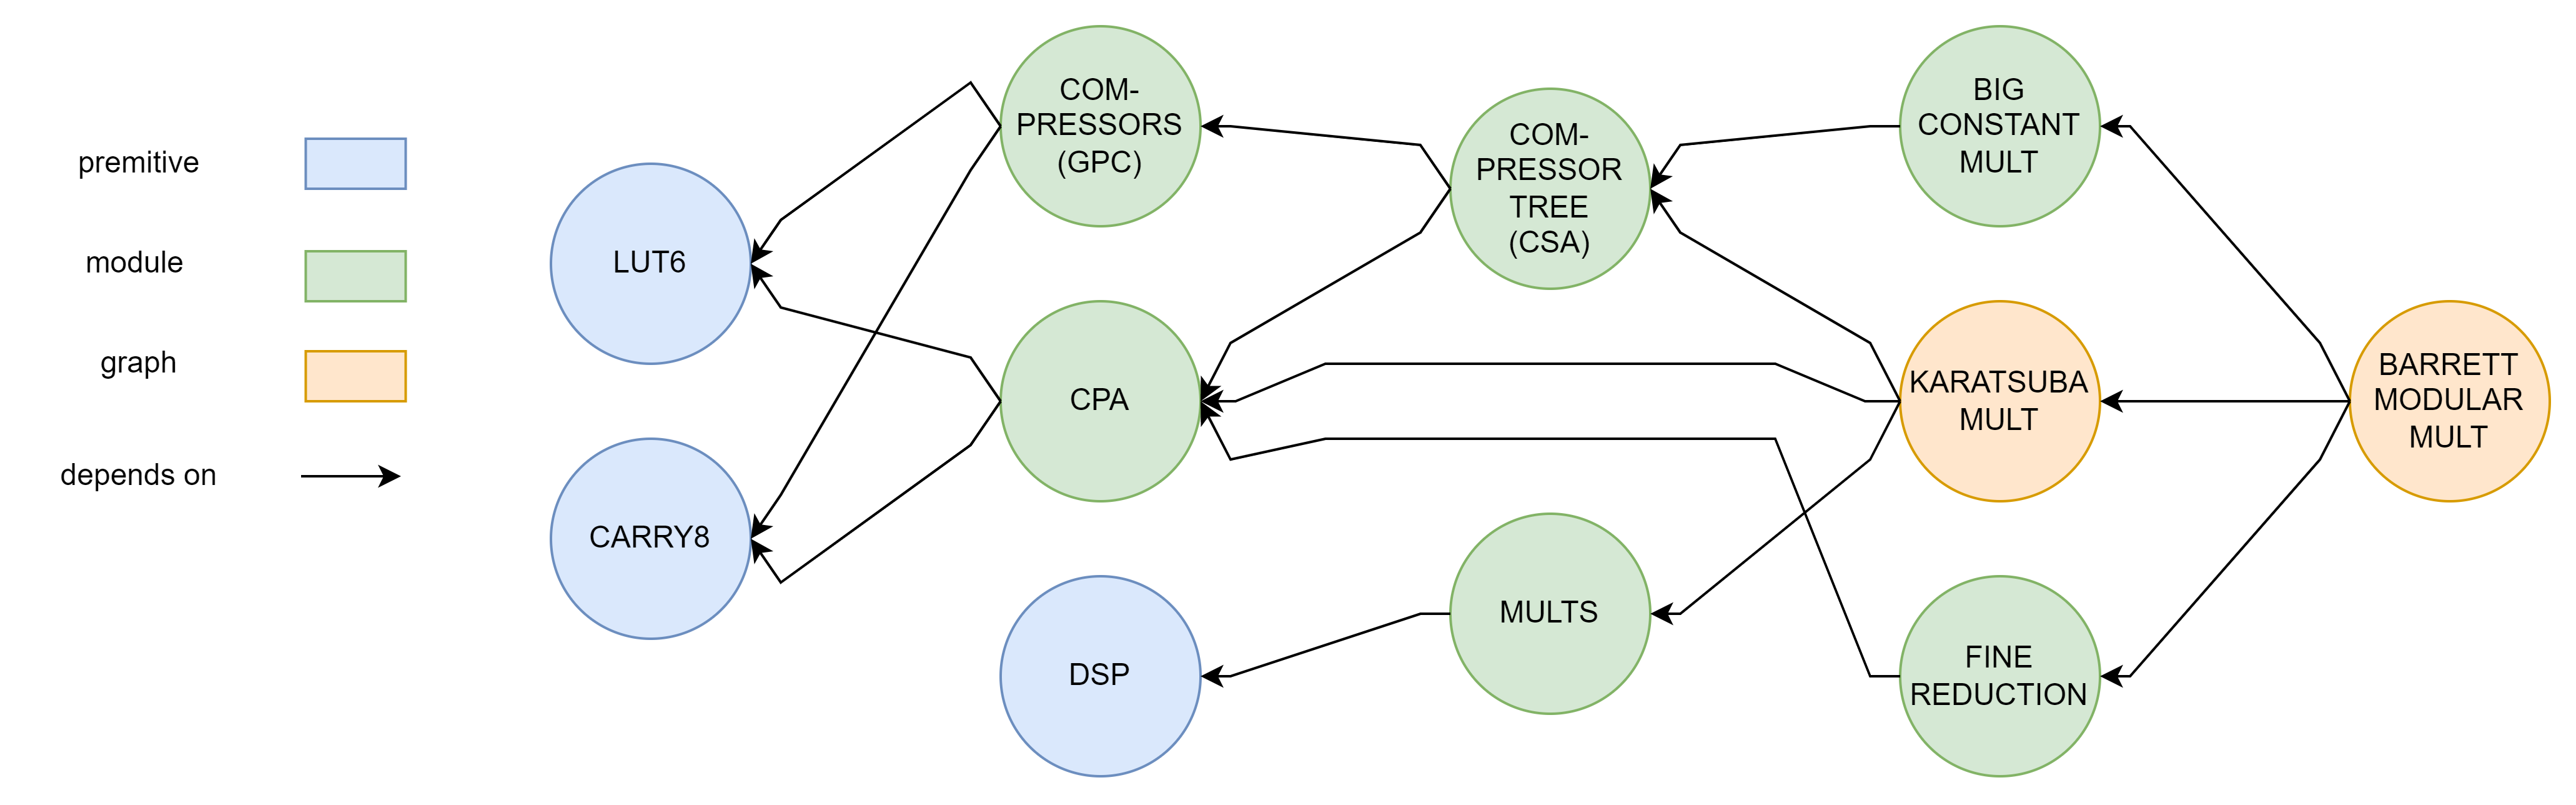
\includegraphics[width=\linewidth,scale=1.00]{fig13.png}    %[]里面的参数自己可根据需要调整
% 	\caption{Please write what you want.}
% 	\label{Figure13}
% \end{figure}

\textcolor{black}{
CSD encoding brings negative bits, which are handled by inverting the negative bits and adding them to the compression tree(Figure \ref{Figure10}). Inverting a negative operand with width $w$ brings a fixed deviation value of $2^w - 1$. All deviations can be determined during compilation, so we first sum the deviations up and then compensate them uniformly by a three-input CPA at the end of the compression tree. In addition, for constant multiplication, the inverse operation is performed only once, since all bits come from its multiplicand.
}


\begin{figure}[htbp]   %单栏图片用{figure}; 双栏用{figure*},加个星号
	\centering
	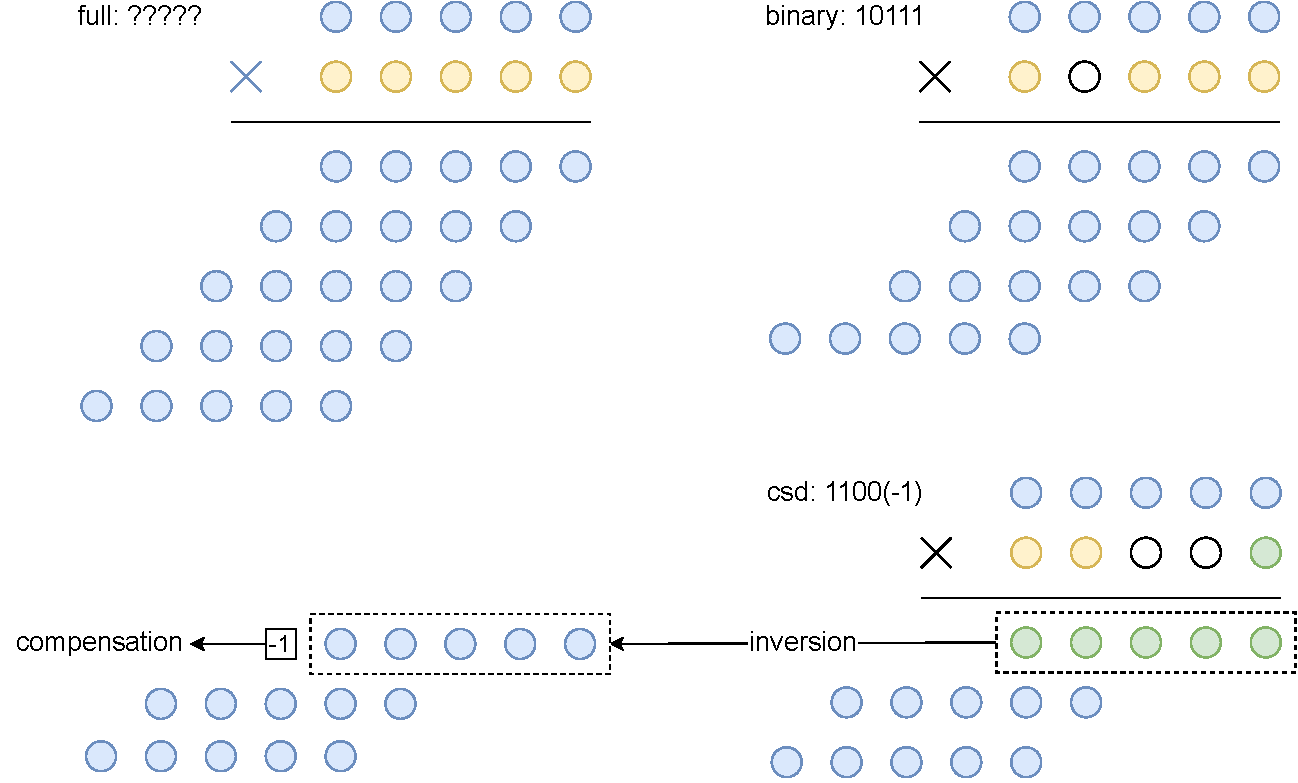
\includegraphics[width=\linewidth,scale=1.00]{fig10.pdf}    %[]里面的参数自己可根据需要调整
	\caption{Implementation of long constant multiplier by compressor tree and CSD encoding.}
	\label{Figure10}
\end{figure}


\subsection{Barrett's Algorithm Using Truncated Multiplication}%使用截断乘法的Barrett算法

\textcolor{black}{
The Barrett's algorithm using truncated multiplication has been derived and proved in  ~\cite{Efficient_FPGA_Modular_Multiplication_Implementation}. In this paper, we extend this method to a large constant multiplier using CSD encoding. We propose a new algorithm, FineBarrett, and prove the following conclusions:
}

\textcolor{black}{
In the case of using CSD encoding with truncation, the LSB multiplier is still able to obtain correct results.
}

\textcolor{black}{
In the case of using CSD encoding and introducing a signed error for the MSB multiplier, the error can be handled by the compensation method of FineReduction.
}

\begin{figure}[htbp]   %单栏图片用{figure}; 双栏用{figure*},加个星号
	\centering
	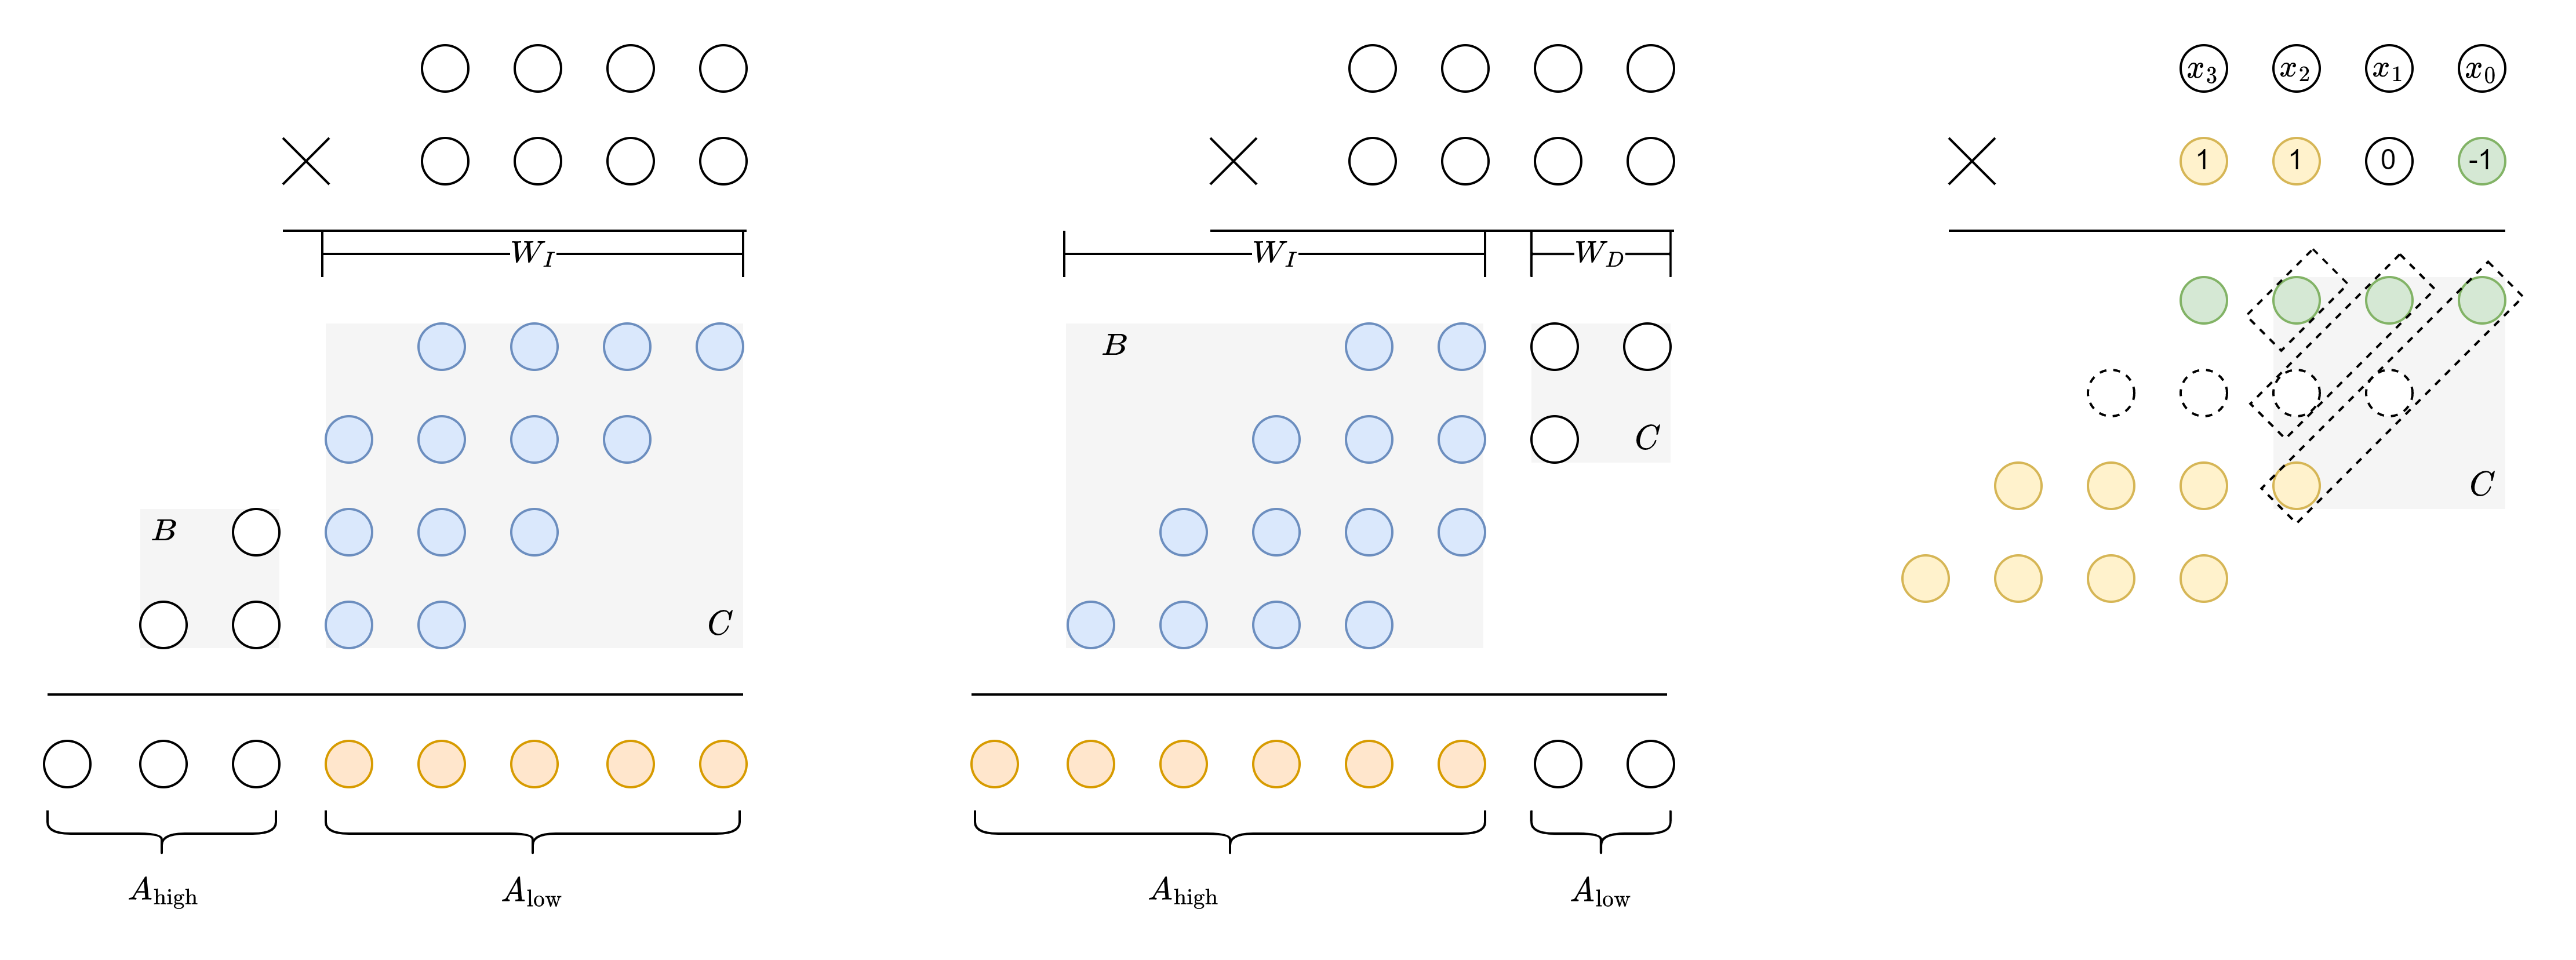
\includegraphics[width=\linewidth,scale=1.00]{fig12.png}    %[]里面的参数自己可根据需要调整
	\caption{Implementation truncated long constant multiplier by CSD encoding.}
	\label{Figure11}
\end{figure}

\textcolor{black}{
In the original Barrett's algorithm, when the input of the constant multiplier is $X$ and the constant is $M$, we denote that $A=XM$. The MSB and LSB multiplication need to calculate the most significant bits $A_{\text{high}}$ and least significant bits $A_\text{low}$ of the result respectively. We perform the MSB and LSB multiplication in the same way as in Figure \ref{Figure11}. We use the position of each bit in the original calculation as the basis. In the MSB multiplication, we discard the bits in the low position, while in the LSB multiplication, we discard the bits in the high position, and the total width of the bits involved in the calculation is denoted as $W_I$.
}


\textcolor{black}{
The sum of the bits involved in the calculation is noted as $C$, and the discarded bits are noted as $B$. From the position of the bits (weights), we have
\begin{equation}
% FIXME: 这里后面考虑下对齐
    \begin{split}
    A = B 2^{W_I} + C = A_{\text{high}}2^{W_I} + A_{\text{low}} \\
    \end{split} 
    \label{basic-decomp}
\end{equation}
}

\begin{equation}
    C \equiv A_{\text{low}}\pmod{2^{W_I}}
    \label{same-mod}
\end{equation}


Since the $W_I$-bit binary adder/subtractor overflows to wrap around to get the result by modular $2^{W_I}$ when not rounding, we just need to use the $W_I$-bit binary adder in the last step of the compression tree to obtain $C' = A_{\text{low}}$, and we note this algorithm as
\begin{equation}
    \text{LSB}^{W_I}_M(X) = XM\mod 2^{W_I}
\end{equation}


For the MSB multiplication, we denote the sum of bits involved in the computation as $B$ and the discarded bits as $C$ (see Figure 12.b) for convenience, so that we can follow the definition in Eq. \ref{basic-decomp}, and we wish to compute the error between the target result $A_{\text{high}}$ and the computed result $B$. From Eq. \ref{basic-decomp}, we have:
\begin{equation}
    \text{error} = A_\text{high} - B = {{C - A_\text{low}}\over{2^{W_D}}}
\end{equation}


By the Eq. \ref{same-mod}, we have:
\begin{equation}
    \text{error} = \lfloor {C \over 2^{W_D}} \rfloor
\end{equation}


The magnitude of the error depends entirely on $C$, and the range of $C$ can be fully determined at compile time, as in Figure \ref{Figure11}:
\begin{equation}
    \begin{split}
    C &= (10\bar{1})_{\text{CSD}}x_0 + (0\bar{1})_{\text{CSD}}x_12^1 + (\bar{1})_{\text{CSD}}x_22^2\\
    &= 3x_0 - 2x_1 - 4x_2
    \end{split} 
\end{equation}


The maximum value is obtained when all bits with positive weights are 1 and all bits with non-negative weights are 0, and vice versa. After the introduction of CSD encoding, the value of $C$ may be negative. We denote the compile-time error range as $[-e_0, e_1]$, where $e_0,e_1 > 0$. In practice, when the target width is $W_T$, we may use a larger $W_I > W_T$ to perform the calculation, noted as $s = W_I - W_T$. The margin of error is then reduced to
\begin{equation}
    [-{\lceil{{e_0}\over 2^s}\rceil}, {\lceil{{e_1}\over 2^s}\rceil}]
\end{equation}


We denote this algorithm as
\begin{equation}
    A_\text{high} - \text{MSB}^{W_I}_M(X) \in [-e_0, e_1], e_0,e_1 \ge 0
\end{equation}


\textcolor{black}{
Still, this range can be fully determined at compile time. Our algorithm FineBarrett, is described in Alg. \ref{alg1}:
}

\begin{algorithm}[ht]
    \caption{FineBarrett} %算法名字
    \label{alg1}
	\LinesNumbered %要求显示行号
    \KwIn{$x,y \in [0, 2^k)$, $M \in [2^{k-1}, 2^k)$, Error tolerance $G$} %输入参数
	\KwOut{$R = xy \mod M$} %输出参数
    Calculate the following while compiling: \;
    $ M' = \lceil {2^{2k} \over M} \rceil$ \;
    $W_0 = k$, $e_1 = \inf$, $e_0 = \inf$ \;
    \While{$e_{1} + e_{0} > G - 3$}{
        Update $e_1$, $e_0$ according to $W_I$ and $M$ \;
        $W_0$ = $W_0$ + 1 \; 
    }
    At the end of the loop, we get $W_0$, $e_0$, $e_1$. \;
    $W_1 = k+ \lceil \log_2(3 + e_1 + e_0)\rceil$ \;
    $\text{comp} = e_0M \mod 2^{W_1}$ \;
     Calculate the following on hardware: \;
     $N = xy$ \;
     $E = \text{MSB}^{W_0}_{M'}(\lfloor {N\over {k+1}} \rfloor)$ \;
     $F =\text{LSB}^{W_1}_M(E)$ \;
     $N_L = N \mod 2^{W_1}$ \;
     $T = (N_L - F + \text{comp}) \mod 2^{W_1}$ \;
     $R =\operatorname{redc}(T)$ \;
\end{algorithm}

\textcolor{black}{
The correctness of the algorithm is proved below: \\
For the original Barrett algorithm, we have $E = \lfloor {N\over {k+1}} \rfloor M', N - ME \in [0, 3M)$~\cite{Efficient_FPGA_Modular_Multiplication_Implementation}. After using the truncated MSB multiplication, we have
\begin{equation}
    N - ME \in [-e_0M, (3+e_1)M)
    \label{range}
\end{equation}
After using the truncated LSB multiplication, we have
\begin{equation}
    F = ME \mod 2^{W_1}
\end{equation}
Notice that $N_L, \text{comp}$ are obtained by $\mod 2^{W_1}$, then
\begin{equation}
    N_L - F + C \equiv (N - ME +e_0M) \mod 2^{W_1}
\end{equation}
By Eq. \ref{range}
\begin{equation}
    N - ME +e_0M \in [0, (3+e_1+e_2)M)
\end{equation}
Since $W_1 = k + \lceil \log_2(3 + e_1 + e_0)\rceil$, we have $2^{W_1} \ge (3+e_1+e_0)2^{k} > (3+e_1+e_0)M$, therefore
\begin{equation}
    \begin{split}
    T =(N_L - F + C) &\mod 2^{W_1} = (N - ME +e_0M) \\
    \mod 2^{W_1} &\equiv xy \mod M
    \end{split} 
\end{equation}
There is also $3 + e_0 + e_1 \le G, T \le 2GM$, by taking $G \le 5$, we can use the fine reduction module in ~\cite{Efficient_FPGA_Modular_Multiplication_Implementation} to find $R$ at the cost of nearly 4 $w_1$-bit subtractors. In the experiment, when using the 377-bit modulus of BLS12-377 in zkSNARK and taking $G = 5$, we can get $W_0 = 382, W_1 = 381$, both MSB multiplication and LSB multiplication are truncated by nearly half of the bits.
}

\subsection{Modular Multiplier Architecture Search}

\textcolor{black}{
The previous discussion of the Karatsuba architecture search can be extended to the modular multiplier level. Our search flow for the modular multiplier architecture is as follows:
\begin{enumerate}[(1)]
    \item According to the variation of modular multipliers, variations of the three multiplier are decided.
    \item The three solutions are searched separately to obtain three Pareto-optimal solution sets (if the implementation is a compressed tree, there is only one solution in the solution set), and the ILP problem is constructed and solved in the same way as before, except that an additional constraint is added so that the total number of implementations of the three multipliers are equal.
\end{enumerate}
}



% \section{PIPELINE MULTIPLIER IMPLEMENTATION}

% \subsection{Pipeline bottleneck}

% \subsection{Improved Implementation of Carry-propagation Adder}

% \subsection{Solving Pipeline by Cross-Boundary Retiming}

\section{EXPERIMENT}

\subsection{Experimental Setup}

\textcolor{black}{
In the experimental part of this paper, we chose three target devices as the hardware platform for the experiment, they are U250, VU9P, Z7020. The reason for choosing them is that the ratio of different resources available for these three devices is different, which is helpful to show the performance of the algorithm for different hardware budgets in the experimental part. In this experiment, our experimental setup is chosen as follows: 
In our experiments, the default configuration of Vivado is used for the synthesis configuration of the target design  (except for the corresponding clock constraints).This experiment was done on a server with Ubuntu 18.04.2 LTS system with AMD Ryzen Threadripper 3960X 24-Core Processor CPU and available memory is 125.74G, and Vivado version is 2021.1 (64bit).Experimental Parameters: The parameters used in this experiment are the parameters of BLS12-177 at 377 bits scale.
}


\subsection{Algorithm Experiments}

\textcolor{black}{
In order to verify that the algorithm proposed in this paper can complete the architecture search in a reasonable time under a certain hardware resource budget, the following two groups of experiments are designed:
\begin{enumerate} %[(1)]
    \item VU9P-oriented search scheme for large number multipliers: The search algorithm is executed by two variants of the large number multiplication, namely, the full multiplication and the square operation. For 4096 bit, the search time of the full multiplier and the square operation are respectively 15259.5246 ms, 1424.873665ms .
    \item VU9P-oriented search scheme modular multiplication: The performance of the search algorithm is verified by searching the modular multiplication of a fixed modulus.For 4096 bit, the search time of the modular multiplier is .
    It is clear that the proposed architecture search algorithm is capable to solve a problem on any available FPGAs in reasonable time.
\end{enumerate}
}

\subsection{Hardware Experiments}

\subsubsection{Variant Gain Experiment}

\textcolor{black}{
In this paper, we introduce a taxonomy of multipliers / modular multipliers as a way to obtain gains in area cost. In the following, we use two different groups of experiments to verify that this classification does result in an area gain:
\begin{enumerate} [(1)]
    \item The area overheads of the three multiplications of FULL-KARATSUBA/FULL-SCHOOLBOOK/SQUARE at 377bit scale, oriented to VU9P, are obtained as shown in Table \ref{377bits-VU9P-Three modular multipliers}. Through the experimental data, it can be proved that the taxonomy of introducing multipliers can bring some gains in area overhead.
    \item At 377bit scale and ZPrize modulus, oriented to VU9P, we implement the three structures of the modular multiplier as 10.a 10.c 10.e, and the area overhead is shown in Table \ref{The area overhead of different modular multiplier structures}.It can be clearly seen from the experimental results that after the application of modular multiplication taxonomy, the area cost of 10.e is the smallest, while that of 10.a is the largest, which reflects the area benefits brought by modular multiplication taxonomy.
\end{enumerate}
}

\begin{table}[]
    \centering
    \caption{Implementation of Three Kinds of Modular Multipliers}
    \renewcommand{\arraystretch}{1.5}
    \begin{tabular}{l|c|c|c}
                \Xhline{1.5pt}
                Multiplier Type    & Bitwidth(bits)   & LUT   & DSP  \\
                \Xhline{1pt}
                FULL-KARATSUBA                            & 377       & 19622 & 162  \\ 
                \Xhline{1pt}
                FULL-SCHOOLBOOK                            & 377       & 25369 & 288  \\ 
                \Xhline{1pt}
                SQUARE                            & 377       & 14344 & 162  \\ 
                \Xhline{1.5pt}    
    \end{tabular}
    %}
    \label{377bits-VU9P-Three modular multipliers}
\end{table}

\begin{table}[]
    \centering
    \caption{The area overhead of different modular multiplier structures}
    \renewcommand{\arraystretch}{1.5}
    %\setlength{\tabcolsep}{10mm}{
    %\begin{tabular}{m{2cm}<{\centering}|m{2cm}<{\centering}|m{1cm}<{\centering}|m{1cm}<{\c%entering}}
    \begin{tabular}{l|c|c|c}
                \Xhline{1.5pt}
                Multiplication structure    &  Bitwidth(bits)           &    LUT        &    DSP    \\
                \Xhline{1pt}
                10.a                      &  377       &   54454            &       478    \\ 
                \Xhline{1pt}
                10.c                      &  377       &    39118      &   162      \\ 
                \Xhline{1pt}
                10.e                      &  377       &    44398      &   162    \\ 
                \Xhline{1.5pt}    
    \end{tabular}
    %}
    \label{The area overhead of different modular multiplier structures}
\end{table}



\subsubsection{Architecture Search Experiment}

In order to show that the proposed algorithm has a wide tradeoff range, We verify this through experiments on a group of different devices. The specific experiment content is:
Under the 377bit scale and ZPrize modulus (using 10.c architecture), the modular multiplier search was carried out for VU9P, C1100 and z7020 respectively. The results are shown in Table \ref{performance of various FPGAs}. It contains the budget of hardware resources, the number of optimal solutions for different Pareto, and the proportion of resource proportion of LUT and DSP. From the analysis of the experimental results, it can be seen that the proposed architecture search algorithm can find as many Pareto optimal solutions as possible under a given constraint and solve for the number of applied solutions according to the corresponding budget to maximize the achievable units.

\begin{table}[h]
    \centering
    \caption{the modular multiplier performance of various FPGAs}
    \renewcommand{\arraystretch}{2}
    %\setlength{\tabcolsep}{10mm}{
    %\begin{tabular}{m{2cm}<{\centering}|m{2cm}<{\centering}|m{1cm}<{\centering}|m{1cm}<{\c%entering}}
    \begin{tabular}{l|c|c|c|c|c|c}
                \Xhline{1.5pt}
                \makecell[c]{Target \\ devices}  &  \makecell[c]{LUT \\ budget} & \makecell[c]{DSP \\ budget}  & Sol.A & Sol.B & \makecell[c]{LUT \\ ratio} &  \makecell[c]{DSP \\ ratio} \\
                \Xhline{1pt}
                VU9P                      &  1182000       &    6840    & 28 & 0 & 97.47$\%$ & 66.31$\%$     \\ 
                \Xhline{1pt}
                C1100                     &  872000       &    5952    & 21 & 0 & 99.09$\%$ & 57.15$\%$       \\ 
                \Xhline{1pt}
                Z7020                     &  85000       &    200    & 1 & 0 & 48.41$\%$ & 81.00$\%$       \\ 
                \Xhline{1.5pt}    
    \end{tabular}
    %}
    \label{performance of various FPGAs}
\end{table}

\subsubsection{Comparison with other works}


In this part of the experiment, We will compare the performance of BLS12-377 with other related work, as follows.


\paragraph {BLS12-177 Performance}
\textcolor{black}{
We chose the BLS12-377 as the test target because the implementation of the BLS12-377 is also discussed in ~\cite{PipeMSM}. Therefore, we can compare it with BLS12-377 to show how much performance improvement in the proposed framework can bring. The result is shown in Table \ref{performance of VU9P under 377 bits}.According to the experimental results, our design can save 35 DSPS on MSB multiplication, and LUT is similar to the resources used in the paper\ref{performance of VU9P under 377 bits}.On the LSB multiplication, we can save 35 DSPS and implement with less LUT.
}
\begin{table}[h]
    \centering
    \caption{Comparison of performance of BLS12-377}
    \renewcommand{\arraystretch}{1.5}
    %\setlength{\tabcolsep}{10mm}{
    %\begin{tabular}{m{2cm}<{\centering}|m{2cm}<{\centering}|m{1cm}<{\centering}|m{1cm}<{\c%entering}}
    \begin{tabular}{l|c|c|c}
                \Xhline{1.5pt}
                Multiplication Type               & Datawidth &   LUT  &  DSP  \\
                \Xhline{1pt}
                MSB multiplication by m           &    377    &    13500    &     35  \\ 
                \Xhline{1pt}
                MSB multiplication by m[proposed] &     377      &  13558      &    0   \\ 
                \Xhline{1pt}
                LSB multiplication by q           &    377    &   10000     &    35   \\ 
                \Xhline{1pt}
                LSB multiplication by q[proposed] &     377      & 9295       &    0   \\ 
                \Xhline{1.5pt}    
    \end{tabular}
    %}
    \label{performance of VU9P under 377 bits}
\end{table}

% \begin{table}[]
%     \centering
%     \caption{xxxx.}
%     \renewcommand{\arraystretch}{1.5}
%     %\setlength{\tabcolsep}{10mm}{
%     %\begin{tabular}{m{2cm}<{\centering}|m{2cm}<{\centering}|m{1cm}<{\centering}|m{1cm}<{\c%entering}}
%     \begin{tabular}{l|c|c|c}
%                 \Xhline{1.5pt}
%                 Multiplication Type       &  size           &    LUT &    DSP\\
%                 \Xhline{1pt}
%                 10.a                      &  377 bits       &        &       \\ 
%                 \Xhline{1pt}
%                 10.c                      &  377 bits       &        &       \\ 
%                 \Xhline{1pt}
%                 10.e                      &  377 bits       &        &       \\ 
%                 \Xhline{1pt}
%                 10.a                      &  Zprice modulus &        &       \\ 
%                 \Xhline{1pt}
%                 10.c                      &  Zprice modulus &        &       \\ 
%                 \Xhline{1pt}
%                 10.e                      &  Zprice modulus &        &       \\ 
%                 \Xhline{1.5pt}    
%     \end{tabular}
%     %}
%     \label{performance of VU9P under 10.x}
% \end{table}



% \begin{table}[]
%     \centering
%     \caption{xxxx.}
%     \renewcommand{\arraystretch}{1.5}
%     %\setlength{\tabcolsep}{10mm}{
%     %\begin{tabular}{m{3.5cm}|m{1.5cm}<{\centering}|m{1.5cm}<{\centering}}
%     \begin{tabular}{l|c|c}
%                 \Xhline{1.5pt}
%                 Multiplication Type             &  LUT      & DSP  \\
%                 \Xhline{1pt}
%                 MSB multiplication by $m$       &  13500    &  35    \\ 
%                 \Xhline{1pt}
%                 LSB multiplication by $q$       &  10000    &  35    \\ 
%                 \Xhline{1.5pt}    
%     \end{tabular}
%     %}
%     \label{performance of BLS12-177}
% \end{table}

%%%%%%% -- PAPER CONTENT ENDS -- %%%%%%%%


% FIXME: 
% ~\cite{Multiplication_of_multidigit_numbers_on_automata}
% ~\cite{UltraScale_Architecture_DSP_Slice_User_Guide}
% ~\cite{Implementing_the_Rivest_Shamir_and_Adleman_public_key} % barrett
% ~\cite{montgomery}


%%%%%%%%% -- BIB STYLE AND FILE -- %%%%%%%%
\bibliographystyle{IEEEtranS}
\bibliography{refs}
%%%%%%%%%%%%%%%%%%%%%%%%%%%%%%%%%%%%


\end{document}